\chapter{Interpretations: 3rd generation squarks}
    \label{chapter:Interpretations}

In this chapter, the model independent upper limits on the visible cross section are presented for the monojet analysis.
The monojet results are then interpreted in terms of searches for new physics in different models with stops or sbottoms in the final state.
When it is possible, these interpretations are then compared to the bounds set by other searches.


\section{Model independent upper limits}
    \label{sec:ModelIndependentLimits}

The agreement between the data and the Standard Model predictions for the different selections is interpreted in terms of model independent 95\% confidence level (CL) upper limits on the visible cross section.
The visible cross section, $\sigma_{\text{vis}}$, is defined as:

\begin{equation}
\sigma_{\text{vis}} = A\times\epsilon\times\sigma = N / L,
\label{eq:visibleXSec}
\end{equation}

\noindent where $\sigma$ is the production cross section, $A$ is the acceptance of the selection (without considering detector effects), $\epsilon$ is the experimental efficiency to select the signal events, $N$ are the expected events for the process and $L$ is the integrated luminosity.
    
Values of $\sigma \times A \times \epsilon$ in the range between 96~fb and 5.2~fb are excluded at 95\% CL.
The limits are derived with pseudo-experiments and with the asymptotic approximation (see Chapter~\ref{chapter:StatisticalModel}), leading to similar results with both approaches, as shown in Table \ref{tab:modelIndependent}.

\begin{table}[tb]
\begin{center}
\begin{tabular}{cccccc}
\hline
{\bf Signal channel} & & $\mathbf{\langle A\times\epsilon\times\sigma\rangle^{95}_\text{\textbf{obs}}\,\text{\textbf{[fb]}}}$ & $\mathbf{S^{95}_\text{\textbf{obs}}}$ & $\mathbf{S^{95}_\text{\textbf{obs}}}$ & $\mathbf{CL_b}$ \\
\hline
\multirow{2}{*}{M1} & asymp & $95.42$ & $1934.8$ & $1953.6^{847.2}_{291.7}$ & $0.49$ \\
                    & toy   & $96.23$ & $1951.2$ & $1962.0^{839.8}_{319.3}$ & $0.49$ \\
\multirow{2}{*}{M2} & asymp & $28.67$ & $581.4$  & $596.9^{200.4}_{122.7} $ & $0.48$ \\
                    & toy   & $28.36$ & $575.0$  & $590.6^{205.0}_{117.2} $ & $0.48$ \\
\multirow{2}{*}{M3} & asymp & $9.63$  & $195.3$  & $193.9^{68.8}_{54.1}$    & $0.49$ \\
                    & toy   & $9.63$  & $195.3$  & $193.7^{68.7}_{53.2}$    & $0.49$ \\
\multirow{2}{*}{M4} & asymp & $13.16$ & $266.8$  & $262.4^{89.5}_{68.5}$    & $0.52$ \\
                    & toy   & $13.22$ & $268.0$  & $264.4^{90.6}_{70.1}$    & $0.52$ \\
\multirow{2}{*}{M5} & asymp & $5.45$  & $110.5$  & $84.2^{33.0}_{23.3}$     & $0.79$ \\
                    & toy   & $5.45$  & $110.5$  & $84.2^{33.0}_{23.3}$     & $0.79$ \\
\multirow{2}{*}{M6} & asymp & $5.22$  & $105.8$  & $61.7^{21.7}_{16.3}$     & $0.96$ \\
                    & toy        & $5.22$  & $105.8$  & $61.9^{21.2}_{16.1}$     & $0.96$ \\
\hline
\end{tabular}
\end{center}
\caption[Model independent 95\% CL limits for the different signal regions.]{Observed and expected 95$\%$ CL limits on the visible cross section, defined as cross sections times acceptance time efficiency for the different signal selections.}
\label{tab:modelIndependent}
\end{table}


\section{Notes on the computation of the limits}
    \label{sec:ComputationOfLimits}

For the models that will be studied in this chapter, the signal regions M1-M3 are considered (see Section~\ref{sec:EventSelection}), and the one providing the best expected $CL_s$ (best exclusion) is used for the results that are reported.

The computation of the limits for these models is based on the profile likelihood method discussed in Section \ref{sec:StatisticalTreatment}.
A simultaneous fit of the MC expectations to the data in the signal and control regions is performed including statistical and systematic uncertainties.
Uncertainties on the signal acceptance times efficiency, the background predictions and the luminosity are considered, and correlations between systematic uncertainties on signal and background predictions are taken into account.
The fit accounts for any potential contamination of signal events in the control regions which a priory has been estimated to be very small.

A statistical test is performed and the $CL_s$ value is computed for each signal model.
Those signal models with a $CL_s<0.05$ are considered excluded.
Once the $CLs$ values are known for all the signal models generated, a linear interpolation between them in the parameter space is performed, so that a continuous exclusion plane can be generated.


\section{Signal samples simulation}
    \label{sec:SignalSimulation}

The stop pair production with $\stoptocharm$ is simulated using {\madgraph} with one additional jet from the matrix element and \pythia-6 for the showering.
CTEQ6L1 PDFs and AUET2B tune are used for the parton distribution functions and the simulation of the underlying event, respectively.
Cross sections are calculated to NLO in the strong coupling constant, adding the resummation of soft gluon emission at NLO+NLL accuracy.
The renormalization and factorization scales are set to the mass of the stop.
The samples are produced with stop masses between $\unit[100]{GeV}$ and $\unit[400]{GeV}$ and neutralino masses between $\unit[70]{GeV}$ and $\unit[390]{GeV}$.
The difference between the $\stopone$ and the $\ninoone$ masses, $\Delta m$, varies between $\unit[2]{GeV}$ and $\unit[82]{GeV}$, in a maximum step size of $\unit[30]{GeV}$. Cases in which $\Delta m < \unit[2]{GeV}$ have not been considered, since in this regime the stop can become long-lived, leading to different signatures, as for example, the one studied in Ref.~\cite{Johansen:2010ac}.

The stop pair production with $\stopfourbody$ is simulated with the same prescriptions as the $\stoptocharm$ MC simulation.
For this process, samples with stop mass ranges between $\unit[110]{GeV}$ and $\unit[300]{GeV}$ and $\Delta m$ that varies between $\unit[10]{GeV}$ and $\unit[80]{GeV}$ are produced.

Samples with asymmetric decay are generated with $\BR{\stoptocharm}=0.5$ and $\BR{\stopfourbody}=0.5$ for stops with masses $\unit[110]{GeV}$, $\unit[200]{GeV}$, $\unit[250]{GeV}$ and $\unit[300]{GeV}$, and with $\Delta m$ equal to $\unit[10]{GeV}$ and $\unit[80]{GeV}$.
These samples, combined with the $\stoptocharm$ and $\stopfourbody$ exclusive decays, allow to simulate different branching fraction scenarios.

Finally, the sbottom pair production with $\sbottomtob$ is simulated similarly, with sbottom masses between $\unit[100]{GeV}$ and $\unit[350]{GeV}$, and neutralino masses between $\unit[1]{GeV}$ and $\Delta m = \unit[10]{GeV}$.


\section{Systematic uncertainties on the signal}
    \label{sec:SysUncertaintiesSignal}

A complete study on systematic uncertainties, including both experimental and theoretical uncertainties, have been performed for each of the models studied.
Similar systematic effects have been found for all the models.
Here, the uncertainties for the stop pair production model with $\stoptocharm$ are presented.

The experimental uncertainties account for effects related to the estimation of the jet and $\met$ reconstruction, energy scale and resolution, pileup and jet vertex fraction mismodeling, and the luminosity.
These uncertainties introduce variations in the signal yield of the order of 3\% to 7\% depending on the third generation squark and neutralino mass configuration, and the signal selection under consideration.

The theoretical uncertainties account for effects related to the modeling of the processes.
These uncertainties can affect either the acceptance or the cross section of the model.
The theoretical uncertainties on the acceptance are parametrized with nuisance parameters in the fit, in a similar way as the experimental uncertainties are modeled.
Instead, a different procedure is followed to account for the theoretical uncertainties on the cross section.
In this case, the fit is performed three times, for the nominal and for the $\pm 1 \sigma$ variations on this uncertainty.
The theoretical uncertainties affecting the acceptance and the cross section are listed in Tables~\ref{tab:signalsyst_mono} and~\ref{tab:signalxsecuncert} respectively, and include:

\paragraph{Scale variations:} The uncertainties on the factorization and renormalization scales are the dominant theoretical uncertainties and affect mainly the cross section.
They are computed by varying both scales by factors two and one-half.
These uncertainties introduce variations between 13\% and 15\% on the cross section depending on the stop mass.
The effect of these uncertainties on the acceptance is found to be between 1\% and 6\% depending on the stop and neutralino mass configuration and the selection under consideration.

\paragraph{ISR/FSR:} The uncertainty on the modeling of the initial- and final-state radiation (ISR/FSR) is evaluated by varying the parameters that regulate the parton shower in a range that is consistent with the experimental data.
Altogether, these uncertainties introduce a variation between 3\% and 6\% on the cross sections.
The uncertainty on the ISR also introduces variations on the acceptance up to 8\% for configurations in which the masses of the stop and the neutralino are similar, whereas its effect is negligible for configurations in which this mass difference is large.
The FSR uncertainty introduces effects on the acceptance between 1\% and 9\% depending on the stop and neutralino mass configurations and the signal region under study.

\paragraph{PS to ME matching scale:}The impact in the signal yields from the variation of the parton shower to matrix element matching is also considered.
The parameters regulating this matching in the MC generator are varied by a factor of two up and down. 
The effect of this uncertainty on the cross section can be up to 5\%.
This systematic uncertainty also introduces an effect up to 10\% on the signal acceptance, as the leading jet $\pt$ and the $\met$ requirements tighten.

\paragraph{PDF:} The uncertainty due to PDFs are evaluated using the Hessian method described in Ref.~\cite{Pumplin:2001ct} with the PDF error sets associated with CTEQ6L1.
This uncertainty affects the cross section of the model up to 8\%, while its effect is negligible in the acceptance.

\paragraph{}

%--- \ref{tab:signalsyst_mono}
\begin{sidewaystable}[h!]
\begin{center}
\begin{small}
\begin{tabular}{lccccccccc}
\hline\hline
$m_{\tilde{t}}$ / $m_{\tilde{\chi}_1^0}$ [GeV]  & 100 / 70 & 100 / 85 & 100 / 95 & 200 / 125 & 200 / 170 & 200 / 195 & 300 / 240 & 300 / 280 & 300 / 295\\
    \hline
    \multicolumn{10}{c}{Signal Region M1}\\
      \hline
      $\alpha_s$ up/down  & 1.5  ($\pm$ 0.4) &  2.6  ($\pm$ 0.4)  &  4.6   ($\pm$ 0.3)  &  0.3   ($\pm$ 0.6)  &  3.8   ($\pm$ 0.6)  &  4.9   ($\pm$ 0.4)  &  1   ($\pm$ 3)  &  8   ($\pm$ 3) &  4   ($\pm$ 2) \\
        radiation high/low  & 4.2   ($\pm$ 0.4)  &  5.1   ($\pm$ 0.4)  &  4.9   ($\pm$ 0.3)  &  1.6   ($\pm$ 0.6)  &  4.1   ($\pm$ 0.6)  &  3.0   ($\pm$ 0.4)  &  1   ($\pm$ 4)  &  4   ($\pm$ 3)  &  1   ($\pm$ 2)\\
        q cut up/down       &  1.1   ($\pm$ 0.4)  &  0.1   ($\pm$ 0.4)  &  0.6   ($\pm$ 0.3)  &  0.8   ($\pm$ 0.6)  &  0.3   ($\pm$ 0.6)  &  0.6   ($\pm$ 0.4)  &  0   ($\pm$ 3)  &  3   ($\pm$ 3)  &  1   ($\pm$ 2)\\
        renorm./fact. scale up/down &  4.1   ($\pm$ 0.4)  &  5.0   ($\pm$ 0.4)  &  6.3   ($\pm$ 0.3)  &  1.5   ($\pm$ 0.6)  &  2.4   ($\pm$ 0.5)  &  4.5   ($\pm$ 0.4)  &  2   ($\pm$ 3)  &  4   ($\pm$ 3)  &  1   ($\pm$ 2)\\
        \hline
            \multicolumn{10}{c}{Signal Region M2}\\
              \hline
              $\alpha_s$ up/down   &  0   ($\pm$ 1)  &  1   ($\pm$ 1)  &  3   ($\pm$ 1)  &  1   ($\pm$ 1) &  2   ($\pm$ 1)  &  3   ($\pm$ 1)  &  3  ($\pm$ 6)  &  4   ($\pm$ 4)  &  2   ($\pm$ 3)\\
                radiation high/low  &  7   ($\pm$ 1)  &  6   ($\pm$ 1)  &  6   ($\pm$ 1)  &  2   ($\pm$ 1)  & 2   ($\pm$ 1)  &  4   ($\pm$ 1)  &  0   ($\pm$ 6)  &  5   ($\pm$ 4)  &  2   ($\pm$ 3)\\
                q cut up/down       &  0   ($\pm$ 1)  &  1   ($\pm$ 1)  &  1   ($\pm$ 1)  &  1   ($\pm$ 1)  & 1   ($\pm$ 1)  &  1   ($\pm$ 1)  &  0   ($\pm$ 6)  &  12  ($\pm$ 4)  &  0   ($\pm$ 3)\\
                renorm./fact. scale up/down &  5   ($\pm$ 1)  &  5   ($\pm$ 1)  &  5   ($\pm$ 1)  &  3   ($\pm$ 1)  & 3   ($\pm$ 1)  &  4   ($\pm$ 1)  &  7   ($\pm$ 6)  &  1   ($\pm$ 4)  &  5   ($\pm$ 3)\\
                \hline
                \multicolumn{10}{c}{Signal Region M3}\\
                  \hline
                  $\alpha_s$ up/down   &  0   ($\pm$ 2)  &  0  ($\pm$ 2)  &  2   ($\pm$ 1)  &  1   ($\pm$ 2)  &  2   ($\pm$ 2)  &  5   ($\pm$ 1) &  1   ($\pm$ 10)  &  9   ($\pm$ 7)  &  5  ($\pm$ 5)\\
                    radiation high/low  &  8   ($\pm$ 2)  &  8   ($\pm$ 2)  &  9   ($\pm$ 1)  &  1   ($\pm$ 2)  & 4   ($\pm$ 2)  &  5   ($\pm$ 1)  &  9   ($\pm$ 11)  &  4   ($\pm$ 7)  &  7   ($\pm$ 5)\\
                    q cut up/down       &  0   ($\pm$ 2)  &  0   ($\pm$ 2)  &  0   ($\pm$ 1)  &  2   ($\pm$ 2)  & 1   ($\pm$ 2)  &  3   ($\pm$ 1)  &  8   ($\pm$ 10)  &  16  ($\pm$ 7)  &  5   ($\pm$ 5)\\
                    renorm./fact. scale up/down & 6   ($\pm$ 2)  &  5   ($\pm$ 2)  &  8   ($\pm$ 1)  &  3   ($\pm$ 2)  & 5   ($\pm$ 2)  &  5   ($\pm$ 1)  &  18  ($\pm$ 11)  &  3   ($\pm$ 7)  &  1   ($\pm$ 5)\\
                    \hline\hline
                    \end{tabular}
                    \end{small}
                    \end{center}
                    \caption[Impact of several theory uncertainties affecting the acceptance on the signal expectation based on the scalar top quark samples.]
{Impact of several theory uncertainties affecting the acceptance on the signal expectation based on the scalar top quark samples.
                      These uncertainties include: renormalization/factorization scale variation (rows labelled ``renorm./fact. scale up/down''), ISR and FSR variations (rows labelled ``$\alpha_s$ up/down'' and ``radiation high/low''), and matching scale variations (row labelled ``q cut up/down'').
                        All uncertainties are given in \%.}
                      \label{tab:signalsyst_mono}
                      \end{sidewaystable}


%--- \ref{tab:signalxsecuncert}
\begin{table}[tb]
\begin{center}
\begin{tabular}{lcc} 
\hline\hline
Stop mass [GeV] & cross section [pb] & Uncertainty [\%]\\
       \hline
       100 & 560.15496 & 16.16\\
       125 & 197.27047 & 15.79\\
       150 & 80.337867 & 15.66\\
       170 & 42.682289 & 15.37\\
       200 & 18.541757 & 14.99\\
       225 & 9.9200506 & 15.05\\
       250 & 5.5819606 & 14.84\\
       275 & 3.2820286 & 14.83\\
       300 & 1.9985039 & 14.79\\
       350 & 0.8084170 & 14.47\\
       400 & 0.3573548 & 14.41\\
       \hline\hline
\end{tabular}
\end{center}
\caption{Cross section and the corresponding theoretical uncertainty from the
  combination of renormalization/factorization scale, $\alpha_s$, and PDF uncertainties.} 
 \label{tab:signalxsecuncert}
 \end{table}


The $\met$ distributions for the nominal samples and the samples with renormalization/factorization scale variations in the signal region M1 are shown in Figure~\ref{fig:signalscalesysta6}.
Figures~\ref{fig:signalisrsysta6} (\ref{fig:signalfsrsysta6}) show the impact of ISR (FSR) variations in the missing transverse energy.
Finally, Figure~\ref{fig:signalmlmsysta6} shows the $\met$ distribution for the nominal sample and the samples with the matching scale variations.

\begin{figure}[tb]
\begin{center}
  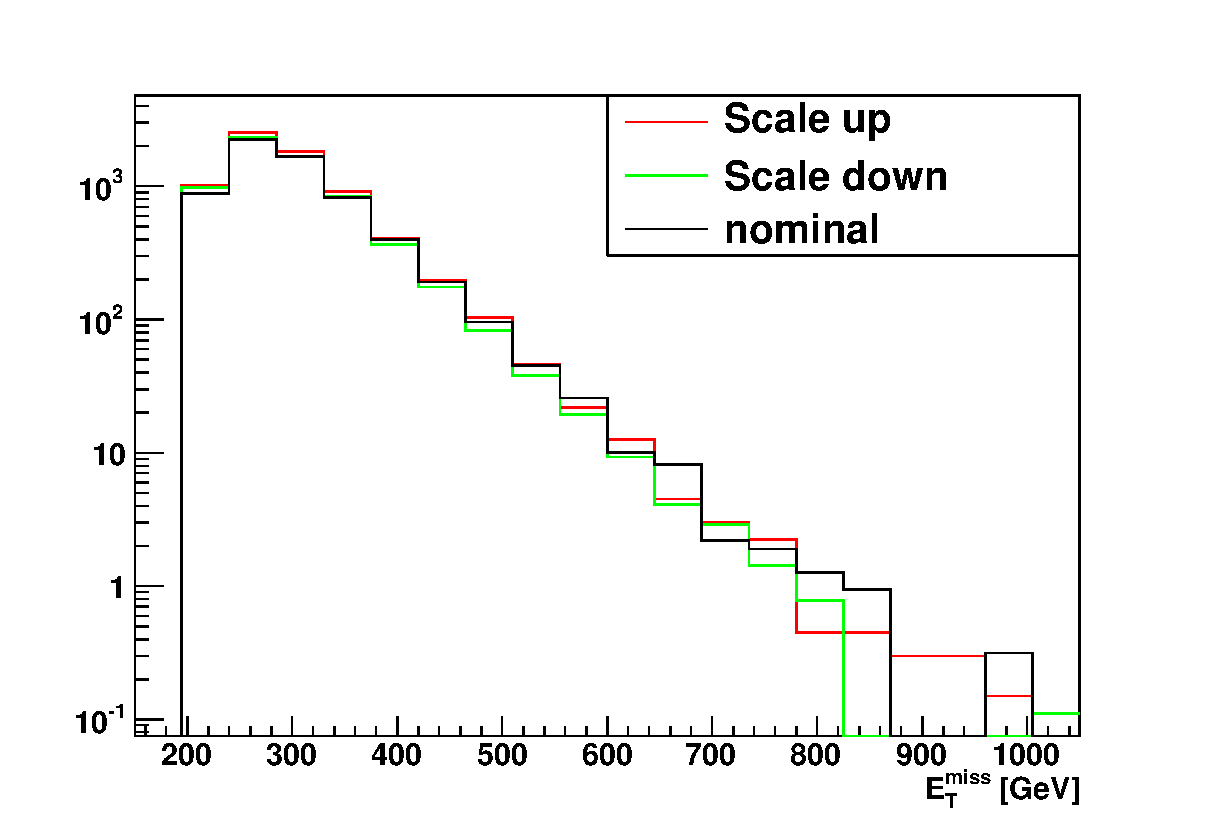
\includegraphics[width=0.49\textwidth]{Interpretations/Figures/stop_100_70_factScale.eps}
  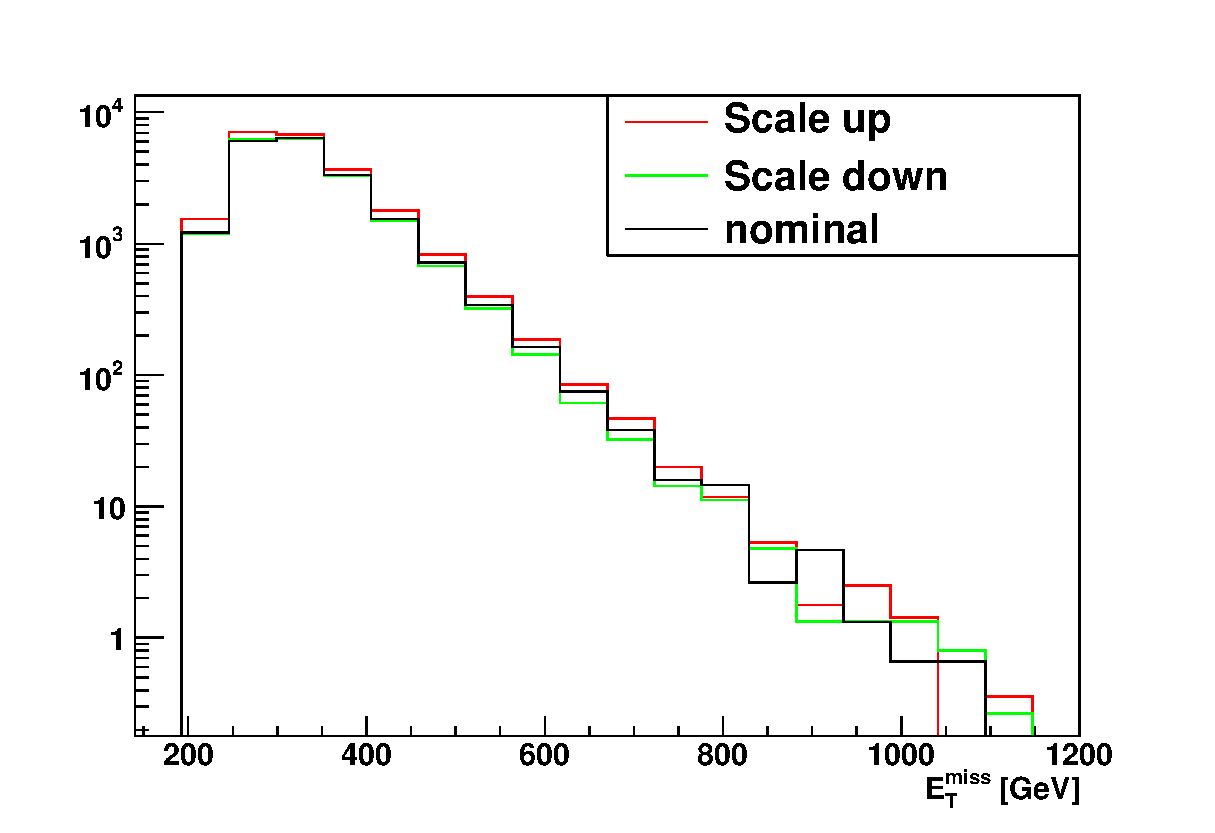
\includegraphics[width=0.49\textwidth]{Interpretations/Figures/stop_100_95_factScale.eps}
  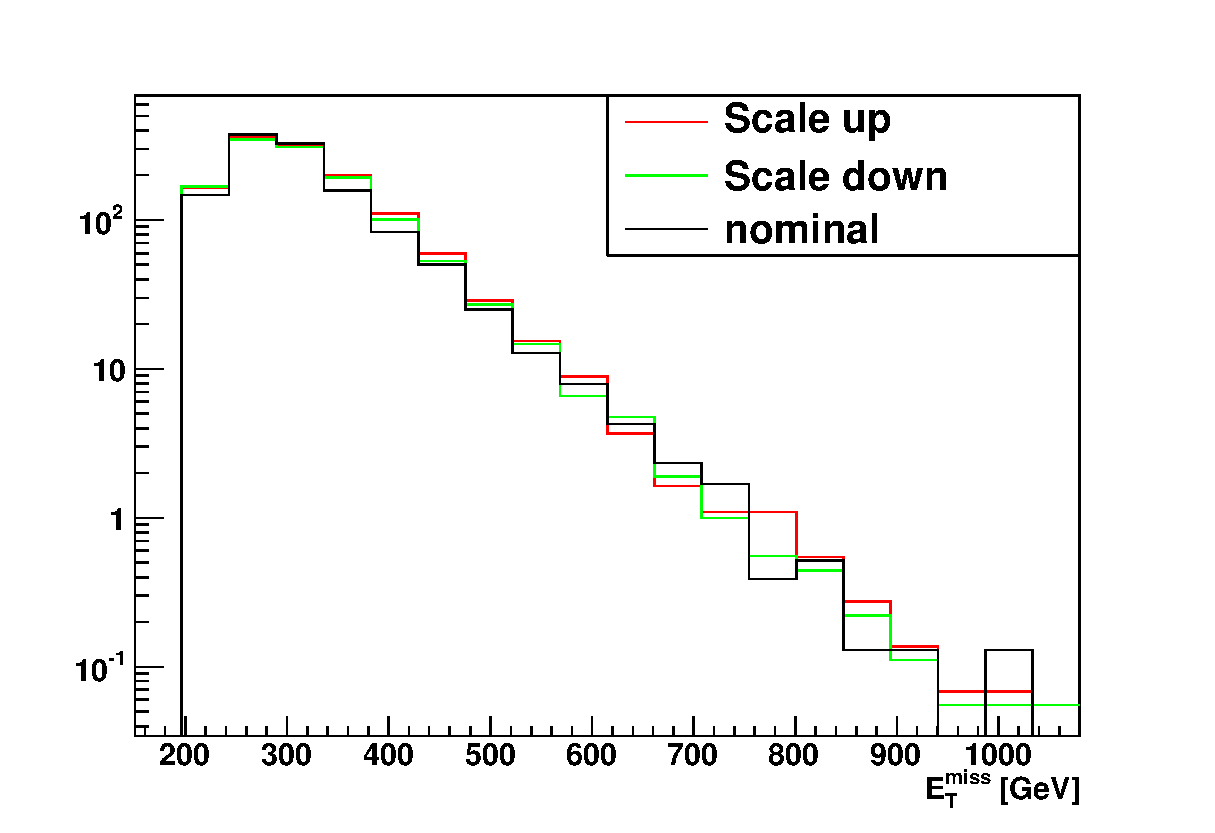
\includegraphics[width=0.49\textwidth]{Interpretations/Figures/stop_200_125_factScale.eps}
  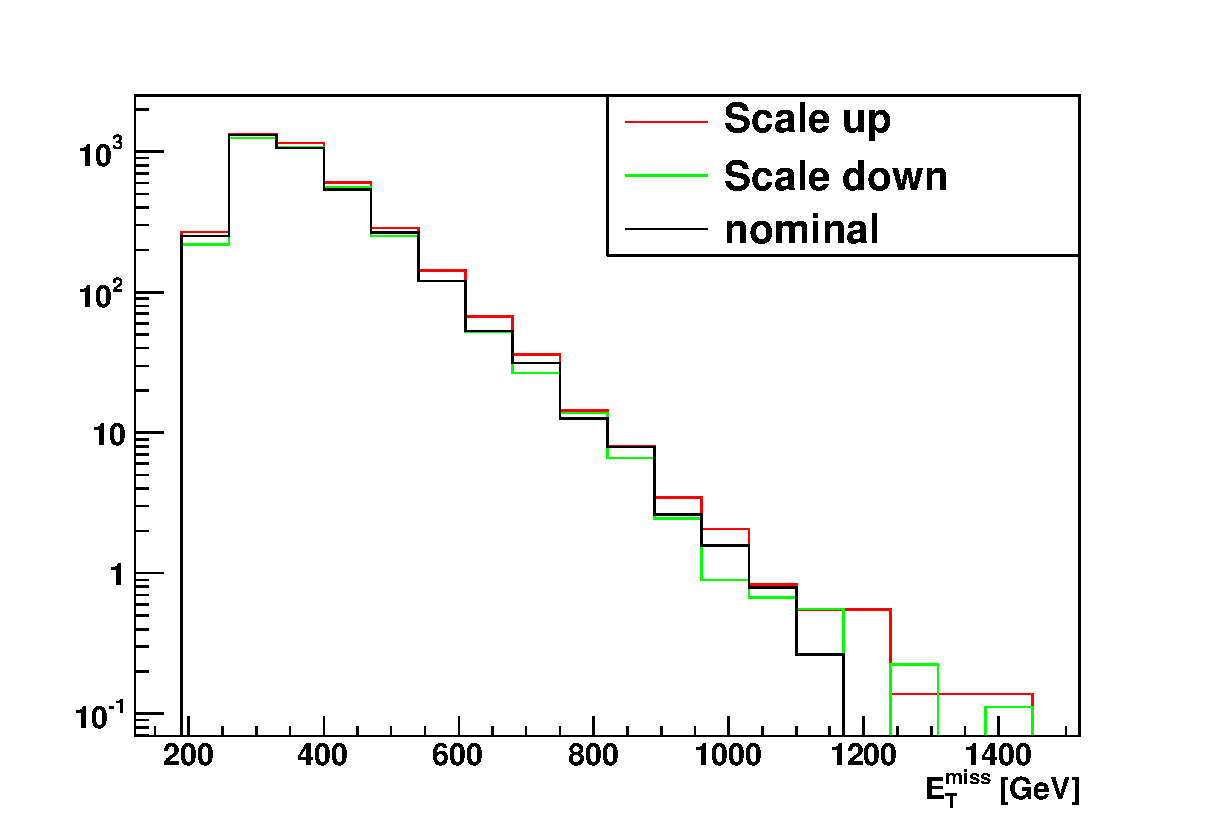
\includegraphics[width=0.49\textwidth]{Interpretations/Figures/stop_200_195_factScale.eps}
\end{center}
\caption[Impact of the renormalization/factorization scale uncertainties on several signal models.]{Impact of the renormalization/factorization scale uncertainties on the missing transverse
  energy for a signal with a scalar
  stop mass of $m_{\tilde{t}}$ = 100\,GeV\ and LSP mass of
  $m_{\tilde{\chi}^0_1}$ = 70\,GeV\ (top left), $m_{\tilde{t}}$ = 100\,GeV\ and
  $m_{\tilde{\chi}^0_1}$ = 95\,GeV\ (top right), $m_{\tilde{t}}$ = 200\,GeV\ and
  $m_{\tilde{\chi}^0_1}$ = 125\,GeV\ (bottom left) and $m_{\tilde{t}}$ = 200\,GeV\ and
  $m_{\tilde{\chi}^0_1}$ = 195\,GeV\ (bottom right).  All plots are
  shown for signal region M1.} 
\label{fig:signalscalesysta6}
\end{figure}

\begin{figure}[tb]
\begin{center}
  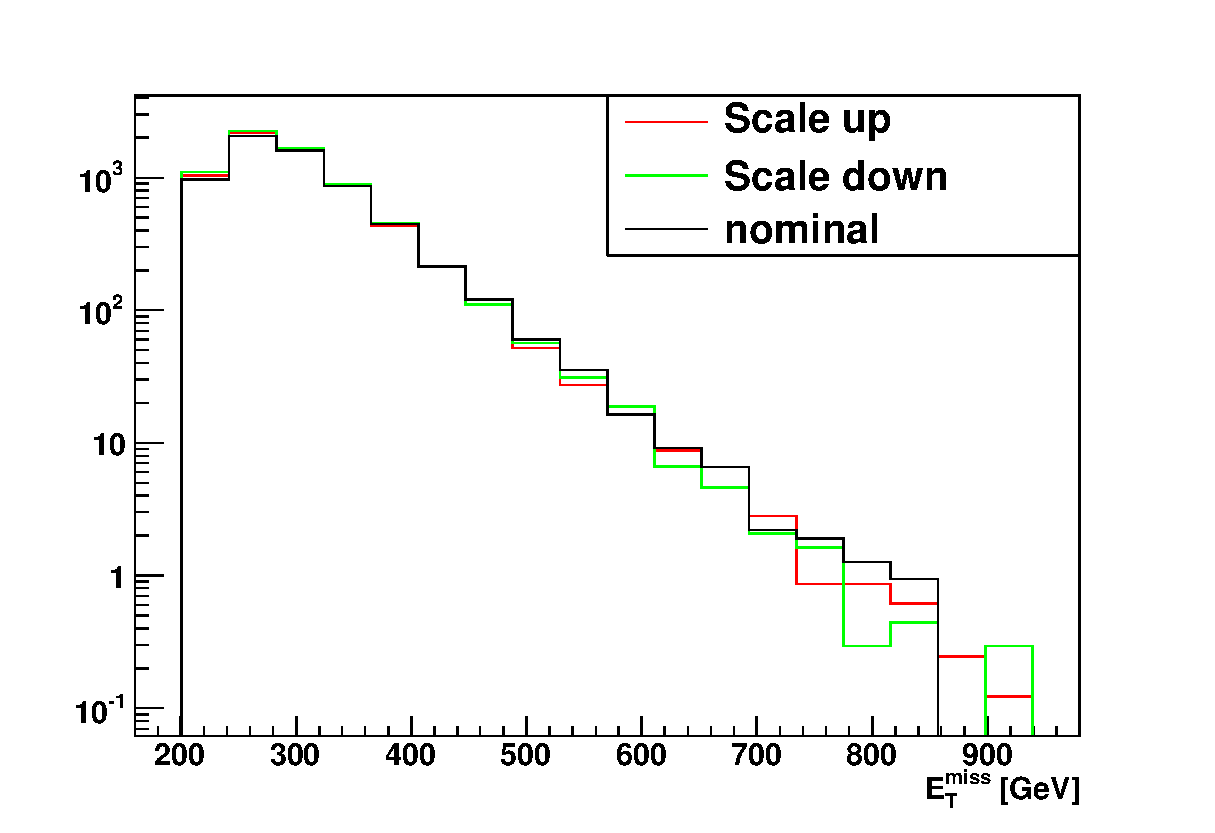
\includegraphics[width=0.49\textwidth]{Interpretations/Figures/stop_100_70_Alpha_s.eps} 
  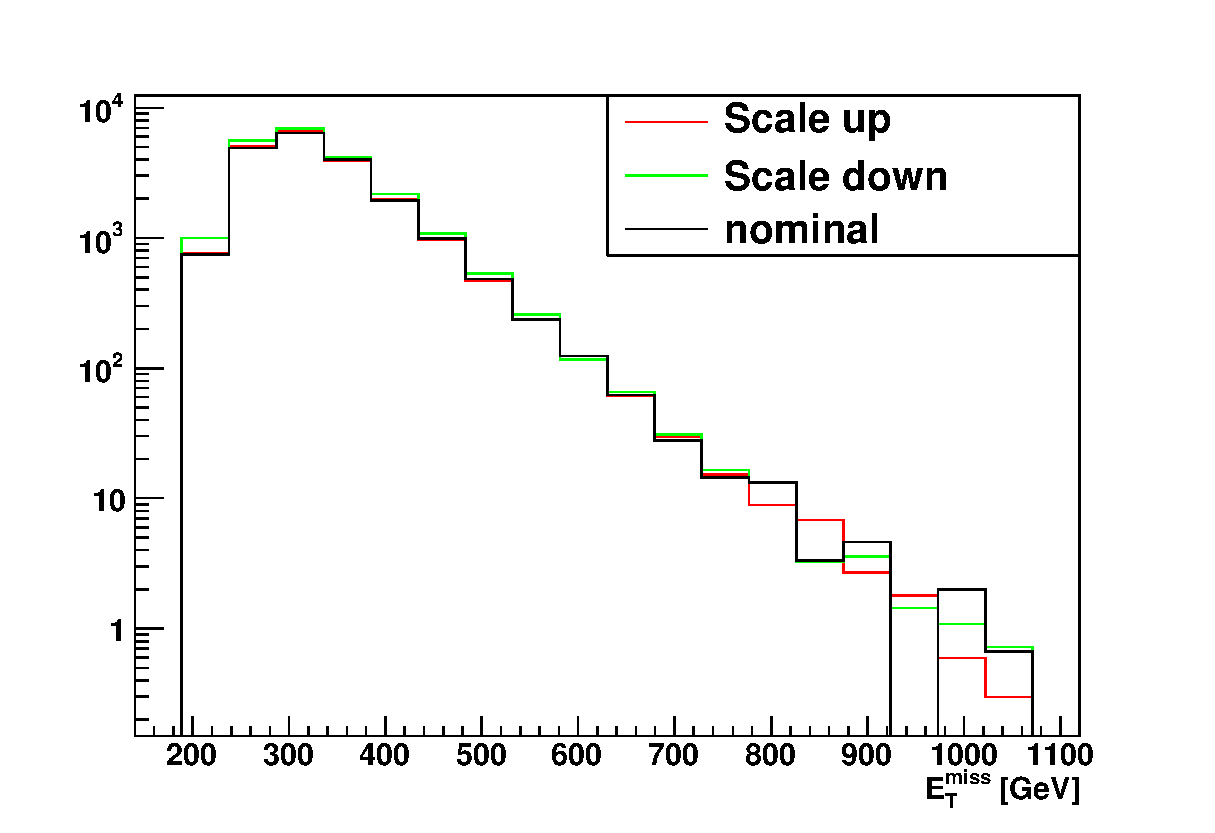
\includegraphics[width=0.49\textwidth]{Interpretations/Figures/stop_100_95_Alpha_s.eps} 
  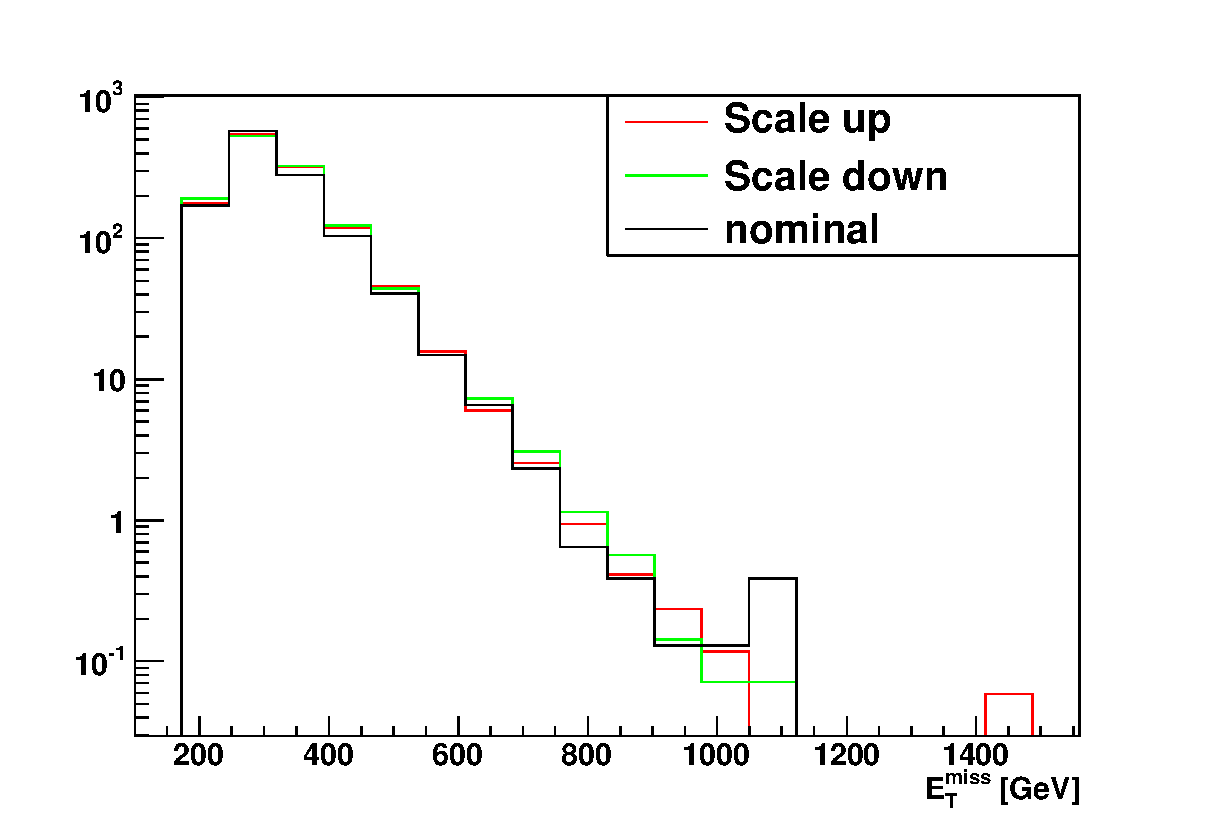
\includegraphics[width=0.49\textwidth]{Interpretations/Figures/stop_200_125_Alpha_s.eps}
  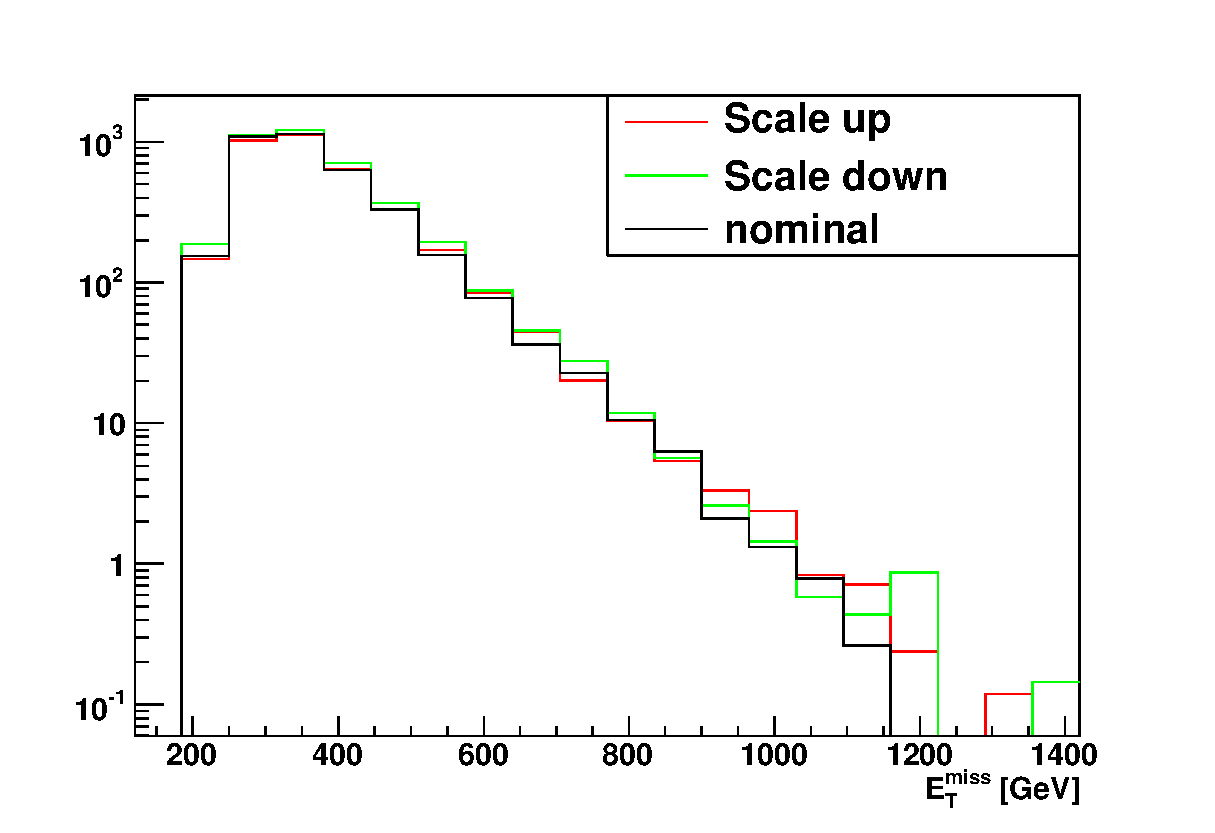
\includegraphics[width=0.49\textwidth]{Interpretations/Figures/stop_200_195_Alpha_s.eps}
\end{center}
\caption[Impact of the ISR uncertainty on several signal models.]{Impact of the ISR uncertainty on the missing transverse
  energy for a signal with a scalar
  stop mass of $m_{\tilde{t}}$ = 100\,GeV\ and LSP mass of
  $m_{\tilde{\chi}^0_1}$ = 70\,GeV\ (top left), $m_{\tilde{t}}$ = 100\,GeV\ and
  $m_{\tilde{\chi}^0_1}$ = 95\,GeV\ (top right), $m_{\tilde{t}}$ = 200\,GeV\ and
  $m_{\tilde{\chi}^0_1}$ = 125\,GeV\ (bottom left) and $m_{\tilde{t}}$ = 200\,GeV\ and
  $m_{\tilde{\chi}^0_1}$ = 195\,GeV\ (bottom right). All plots are
  shown for signal region M1.}
\label{fig:signalisrsysta6}
\end{figure}

\begin{figure}[tb]
\begin{center}
  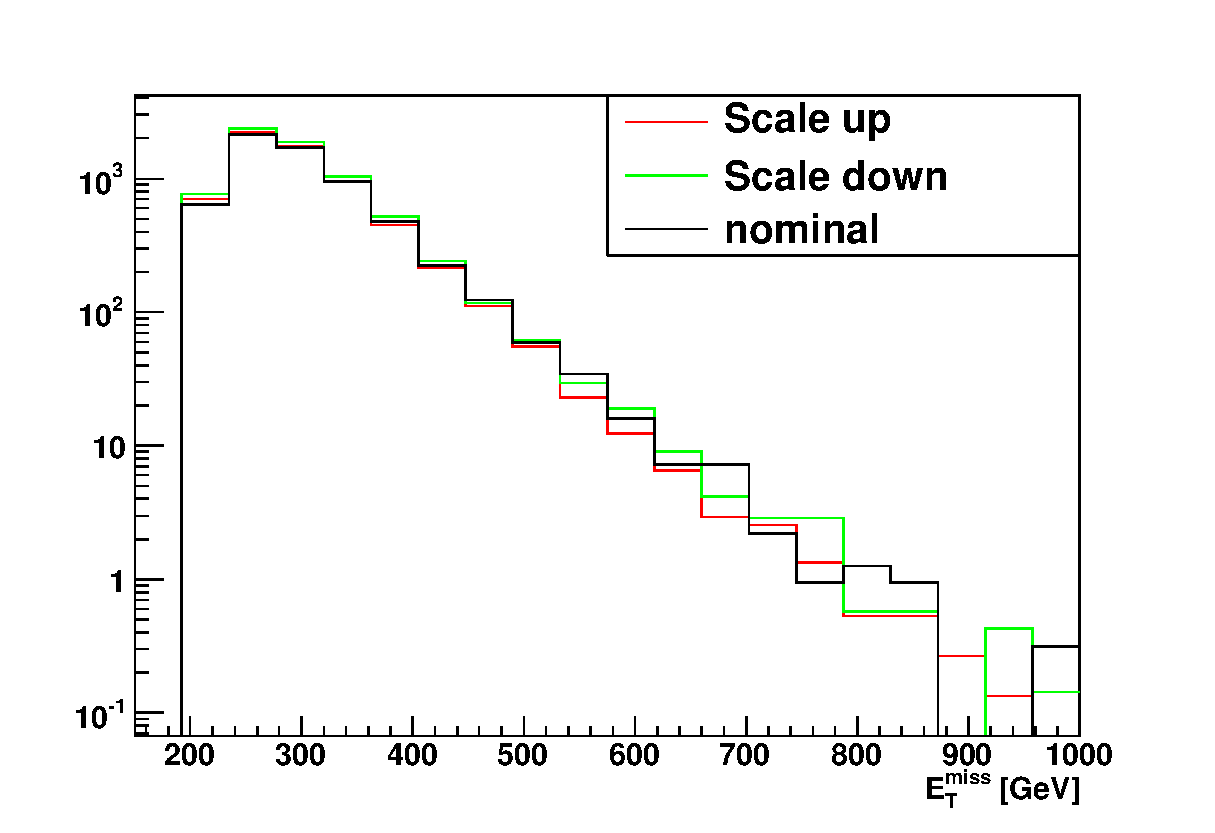
\includegraphics[width=0.49\textwidth]{Interpretations/Figures/stop_100_70_FSR.eps} 
  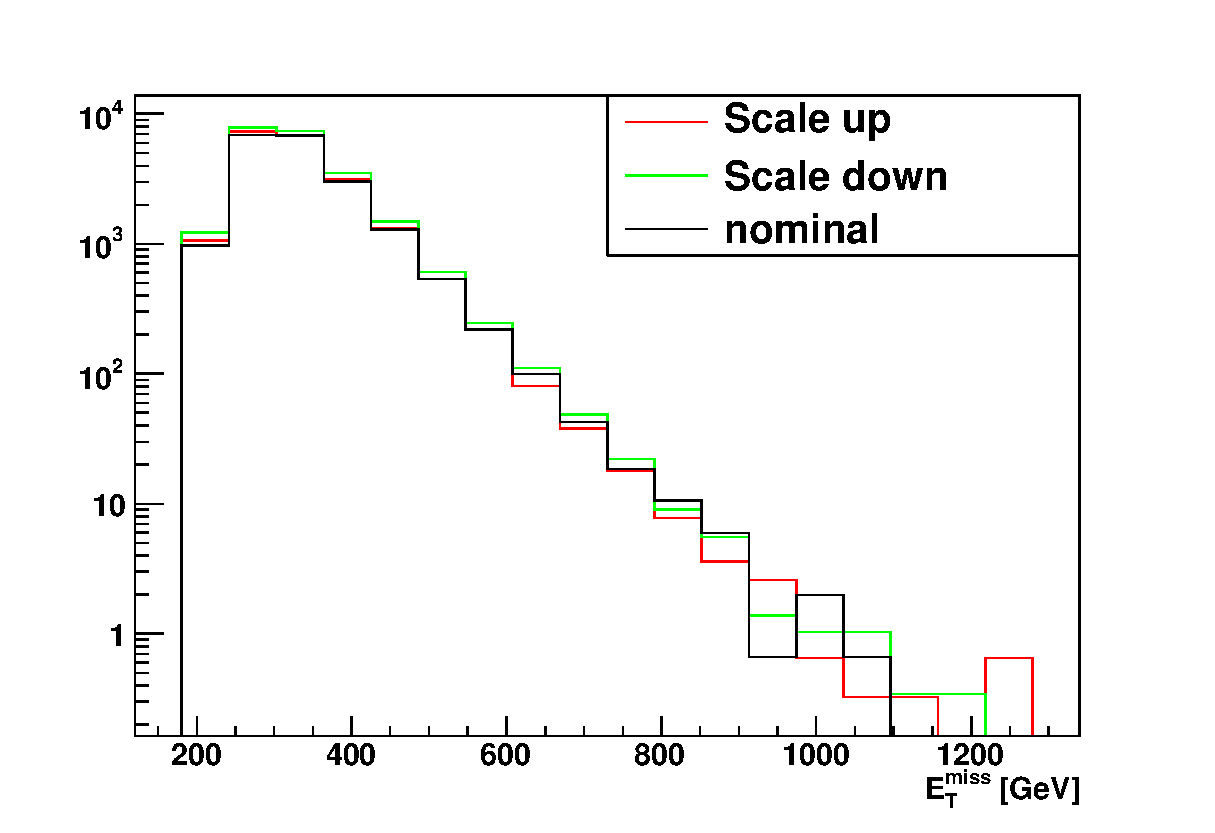
\includegraphics[width=0.49\textwidth]{Interpretations/Figures/stop_100_95_FSR.eps} 
  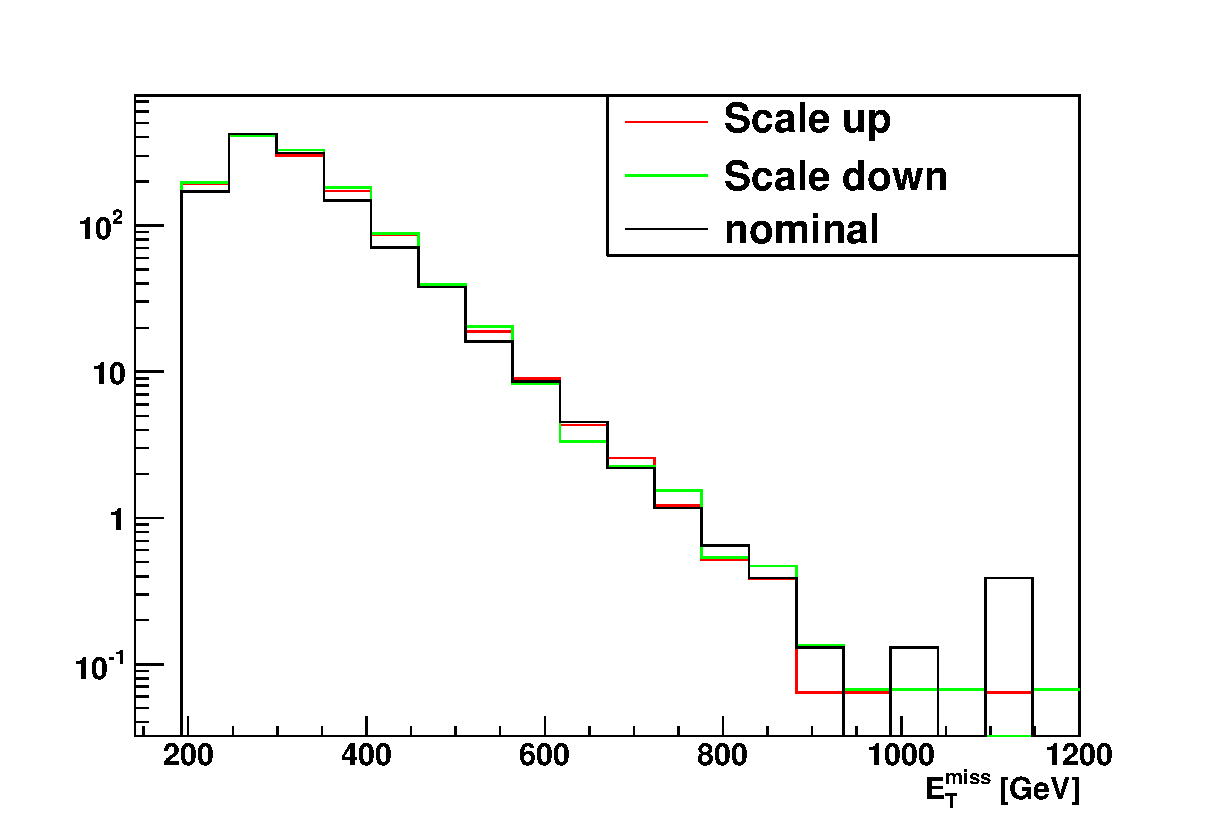
\includegraphics[width=0.49\textwidth]{Interpretations/Figures/stop_200_125_FSR.eps}
  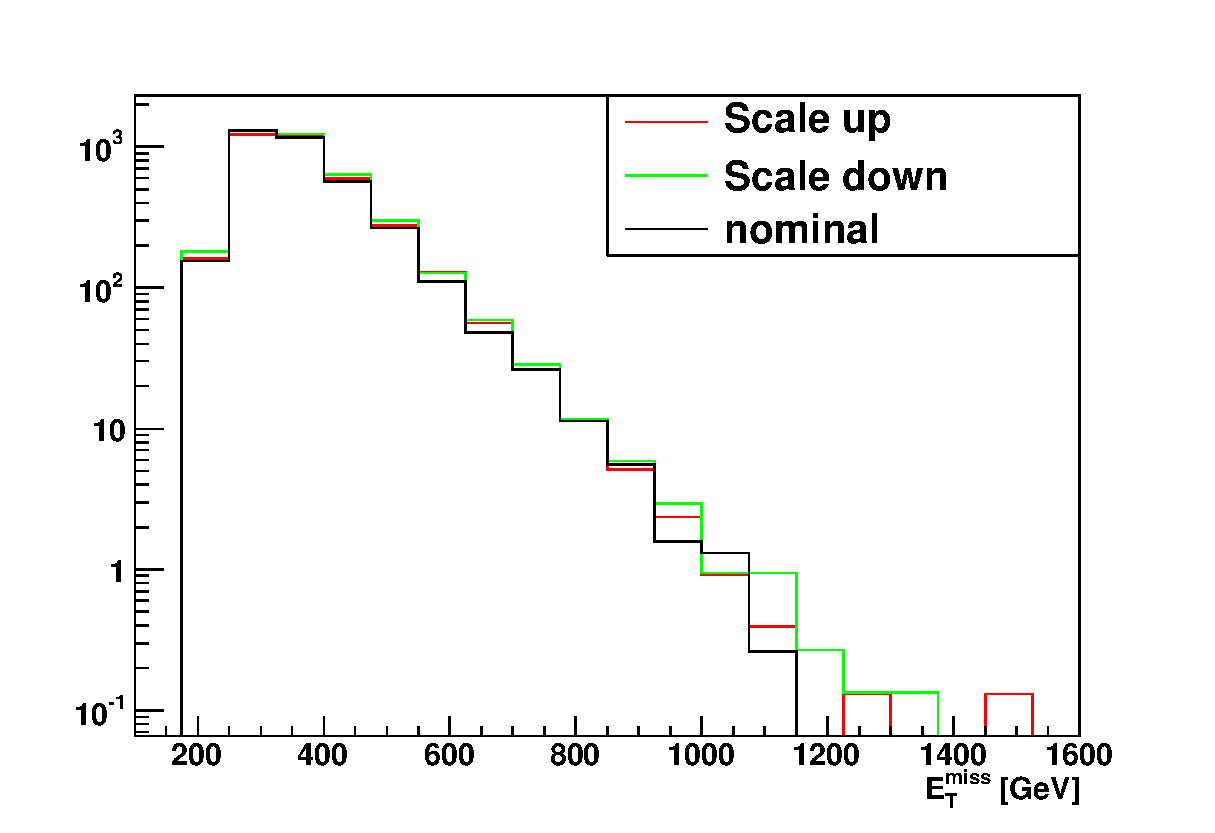
\includegraphics[width=0.49\textwidth]{Interpretations/Figures/stop_200_195_FSR.eps}
\end{center}
\caption[Impact of the FSR uncertainty on several signal models.]{Impact of the FSR uncertainty on the missing transverse
  energy for a signal with a scalar
  stop mass of $m_{\tilde{t}}$ = 100\,GeV\ and LSP mass of
  $m_{\tilde{\chi}^0_1}$ = 70\,GeV\ (top left), $m_{\tilde{t}}$ = 100\,GeV\ and
  $m_{\tilde{\chi}^0_1}$ = 95\,GeV\ (top right), $m_{\tilde{t}}$ = 200\,GeV\ and
  $m_{\tilde{\chi}^0_1}$ = 125\,GeV\ (bottom left) and $m_{\tilde{t}}$ = 200\,GeV\ and
  $m_{\tilde{\chi}^0_1}$ = 195\,GeV\ (bottom right).  All plots are
  shown for signal region M1.}
\label{fig:signalfsrsysta6}
\end{figure}

\begin{figure}[tb]
\begin{center}
  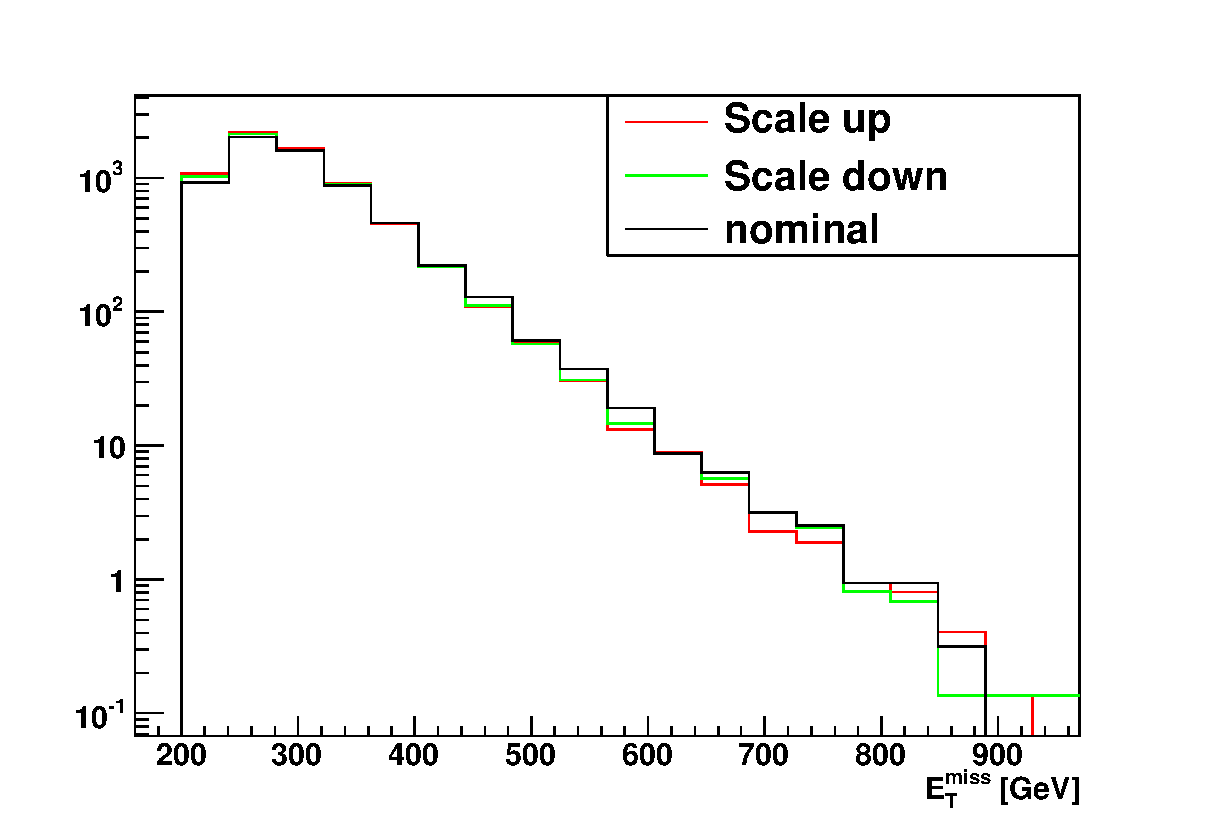
\includegraphics[width=0.49\textwidth]{Interpretations/Figures/stop_100_70_Q.eps} 
  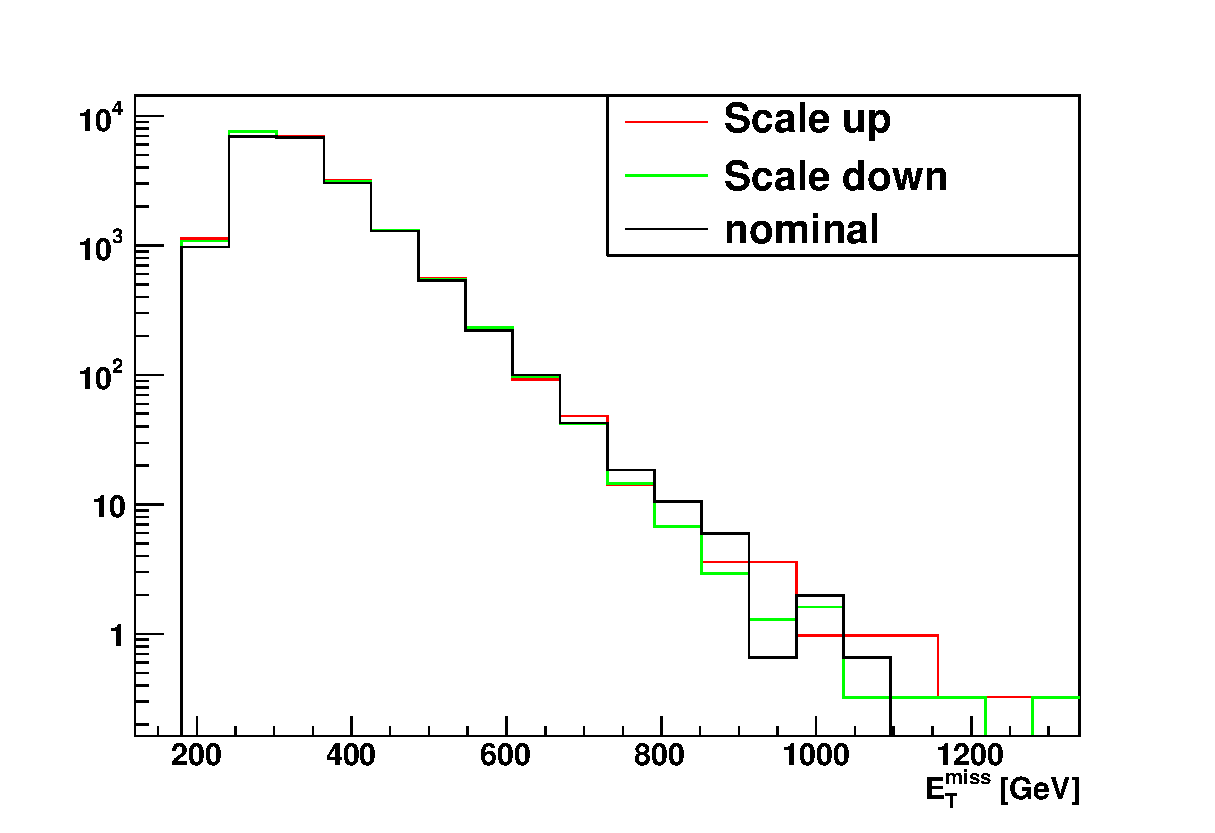
\includegraphics[width=0.49\textwidth]{Interpretations/Figures/stop_100_95_Q.eps} 
  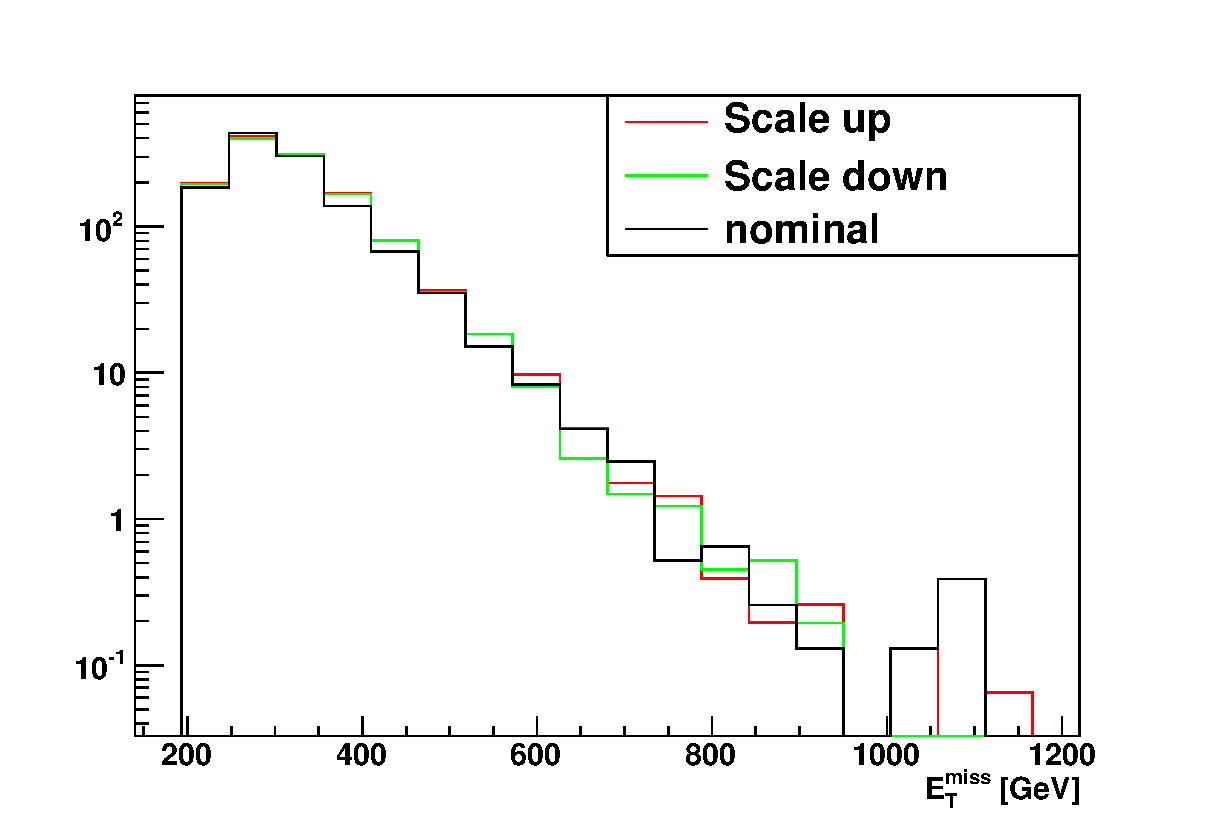
\includegraphics[width=0.49\textwidth]{Interpretations/Figures/stop_200_125_Q.eps}
  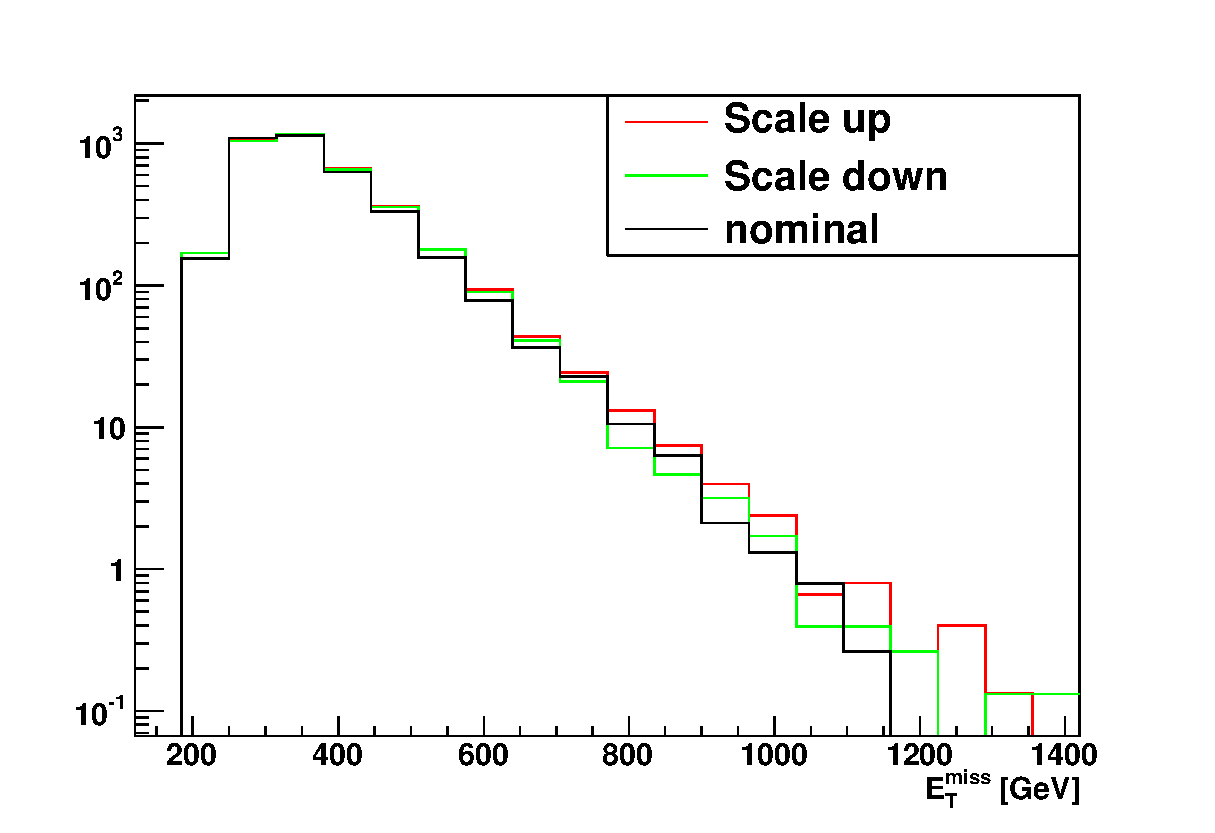
\includegraphics[width=0.49\textwidth]{Interpretations/Figures/stop_200_195_Q.eps}
\end{center}
\caption[Impact of the MLM matching scale uncertainty on several signal models.]{Impact of the matrix element to parton shower matching scale uncertainty on the missing transverse energy for a signal with a scalar
  stop mass of $m_{\tilde{t}}$ = 100\,GeV\ and LSP mass of
  $m_{\tilde{\chi}^0_1}$ = 70\,GeV\ (top left), $m_{\tilde{t}}$ = 100\,GeV\ and
  $m_{\tilde{\chi}^0_1}$ = 95\,GeV\ (top right), $m_{\tilde{t}}$ = 200\,GeV\ and
  $m_{\tilde{\chi}^0_1}$ = 125\,GeV\ (bottom left) and $m_{\tilde{t}}$ = 200\,GeV\ and
  $m_{\tilde{\chi}^0_1}$ = 195\,GeV\ (bottom right).  All plots are
  shown for signal region M1.}
\label{fig:signalmlmsysta6}
\end{figure}


\clearpage
\section{Direct stop pair production}
    \label{sec:DirectStopProduction}

The results of the monojet analysis are translated into exclusion limits on the pair production of top squarks as a function of the stop mass for different neutralino masses.


\subsection{Stop decaying to a charm quark and a neutralino}

In this model, each top squark produced is assumed to decay in a charm-quark and a neutralino, $\stoptocharm$, with a branching fraction of $100\%$.
A Feynman diagram for this process is shown in Figure~\ref{fig:Diagrams3rdGen} (left).
This final state is characterized by the presence of two jets from the hadronization of the charm quarks, and missing transverse energy from the two undetected LSPs.
However, given the relatively small difference between the stop and the neutralino masses, $\Delta m$, both the transverse momenta of the two charm jets and the $\met$ are low, making it very difficult to extract the signal from the large multijet background.
Instead, the presence of initial-state radiation jets is required to boost the squark-pair, leading to larger $\met$.

The monojet analysis is expected to be sensitive in the very low $\Delta m$ region of the phase space, where the charm jets are not boosted enough to be detected.
Figure~\ref{fig:modelIndependent} shows the fiducial cross section, $\sigma\times A \times \epsilon$, as a function of the mass of the stop for different $\Delta m$ configurations in each selection.
For illustration, the model independent limits from Table~\ref{tab:modelIndependent} are included.
The stop and neutralino mass configurations excluded by the monojet analysis can already be approximately inferred from this figure.

\begin{figure}[!ht]
  \begin{center}
    \mbox{
      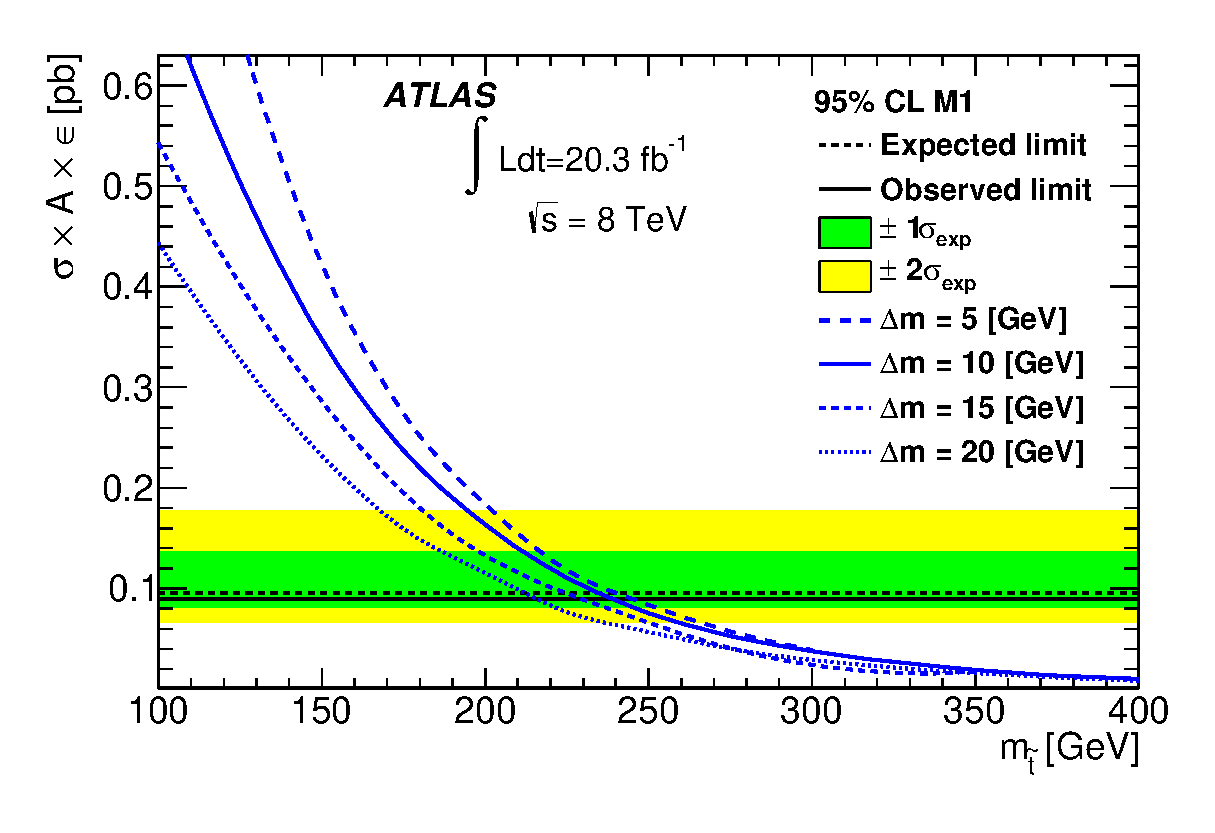
\includegraphics[width=0.495\textwidth]{MonojetAnalysis/Figures/ModelIndependent_Stop_M1.eps}
      \includegraphics[width=0.495\textwidth]{MonojetAnalysis/Figures/ModelIndependent_Stop_M2.eps}
    }
    \mbox{
      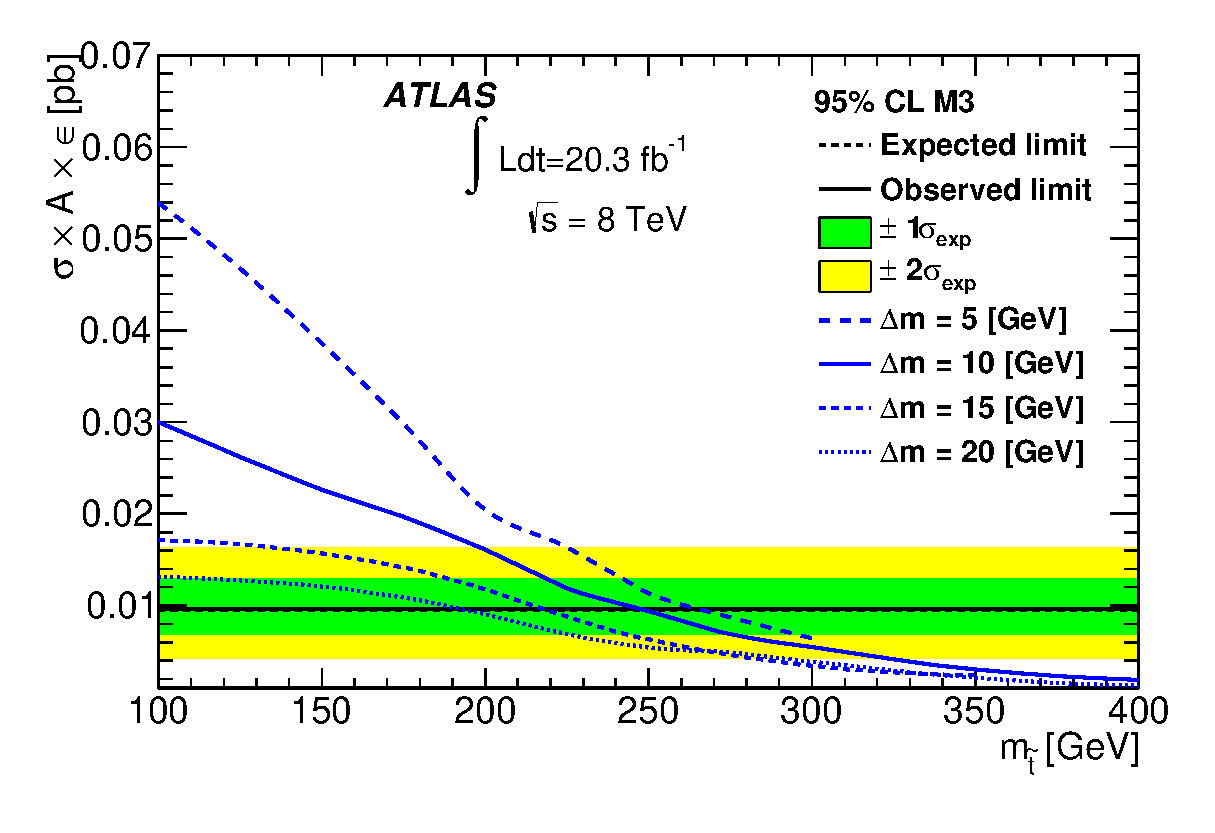
\includegraphics[width=0.495\textwidth]{MonojetAnalysis/Figures/ModelIndependent_Stop_M3.eps}
      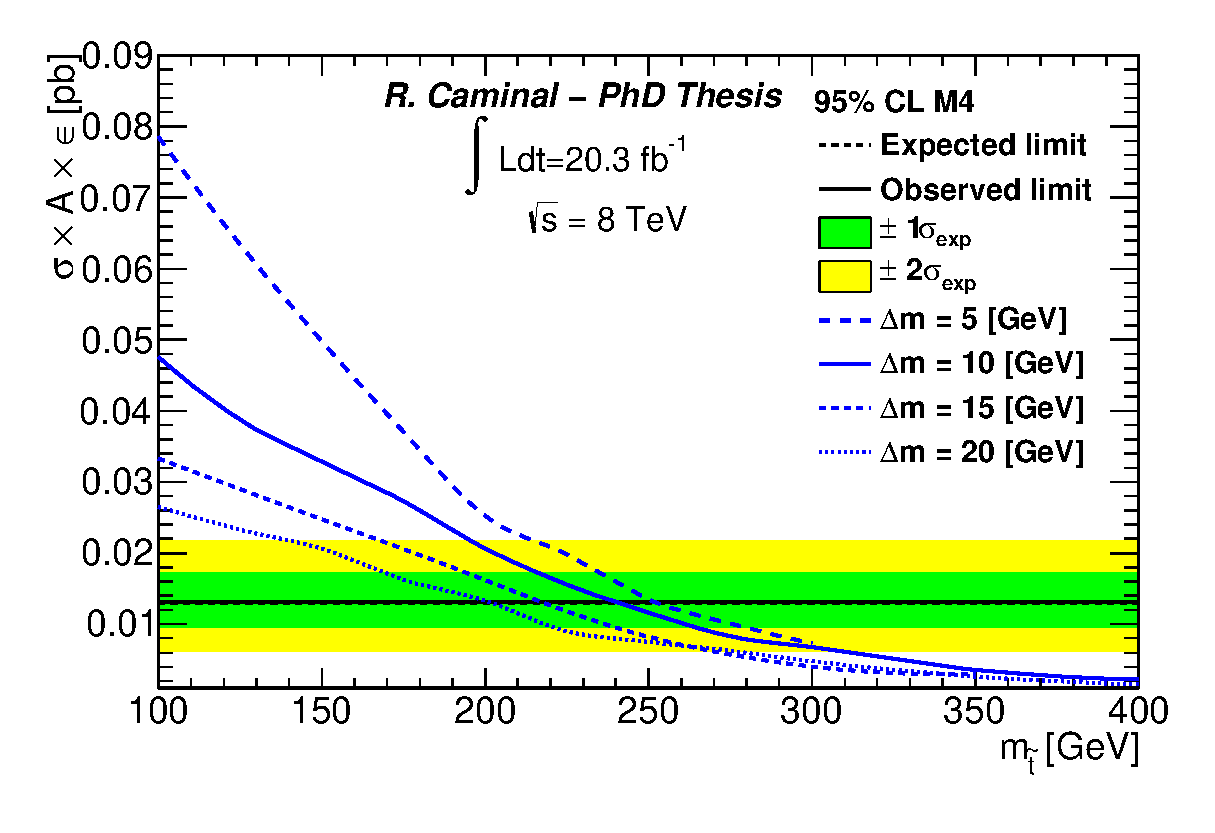
\includegraphics[width=0.495\textwidth]{MonojetAnalysis/Figures/ModelIndependent_Stop_M4.eps}
    }
    \mbox{
      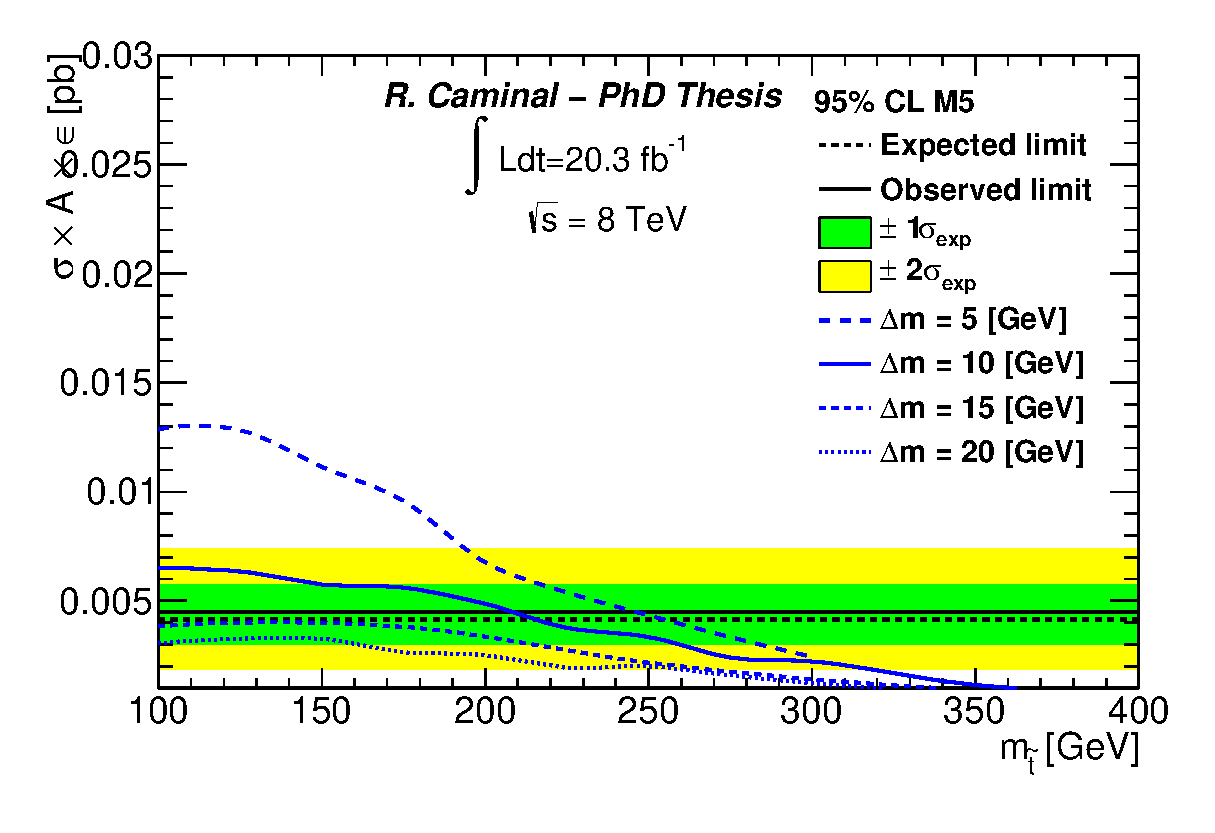
\includegraphics[width=0.495\textwidth]{MonojetAnalysis/Figures/ModelIndependent_Stop_M5.eps}
      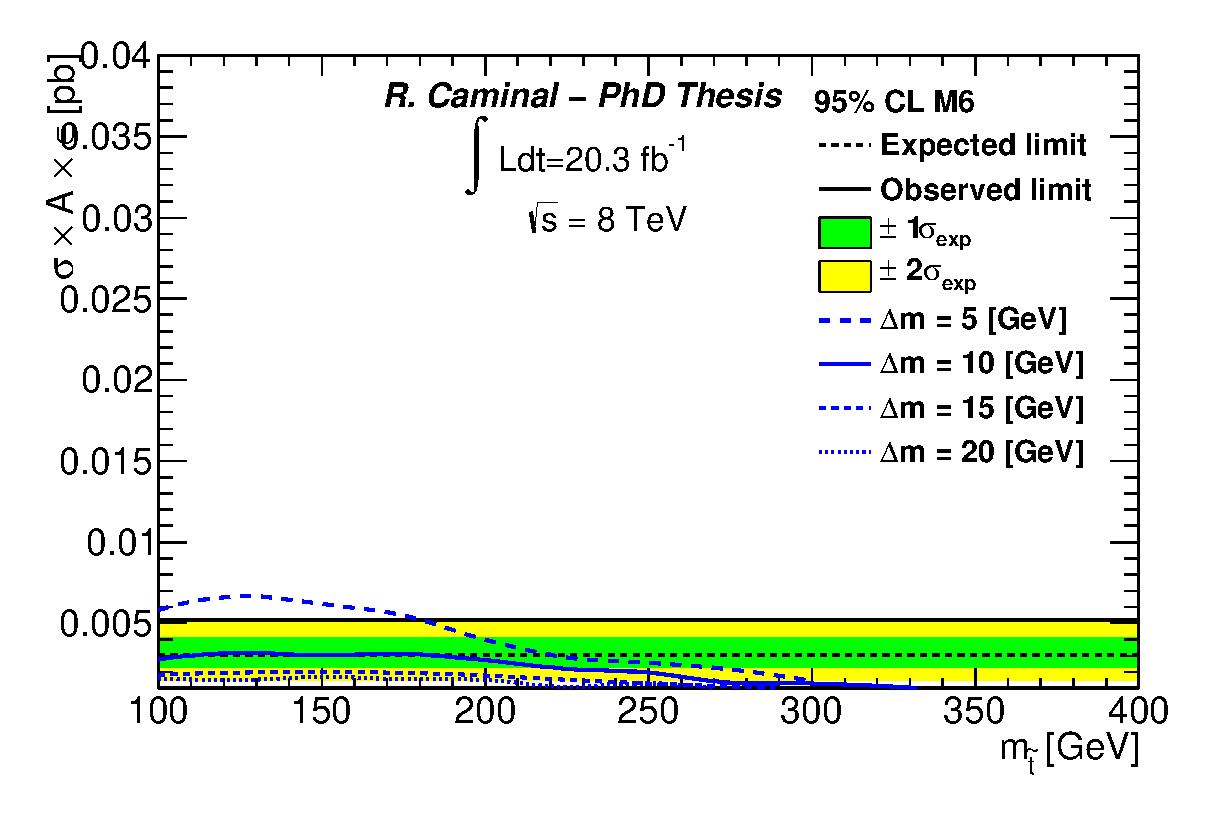
\includegraphics[width=0.495\textwidth]{MonojetAnalysis/Figures/ModelIndependent_Stop_M6.eps}
    }
  \end{center}
  \caption[Model independent 95\% CL limits for the different signal regions.]{Observed and expected 95\% CL model independent limits on the visible cross section for the regions M1-M6 compared to the $\stoptocharm$ predictions as a function of the stop mass for different $\Delta m$.}
  \label{fig:modelIndependent}
\end{figure}

The 95\% CL limits on this model are computed with the $CL_s$ method described in Section~\ref{sec:ComputationOfLimits}, which properly accounts for the correlations on the systematic uncertainties among the different signal and background processes.
Observed and expected limits are computed separately in the different signal regions, and the one with best expected limit is adopted as the nominal result.
The signal region that gives the best expected limit for each stop and neutralino mass is shown in Figure~\ref{fig:ExclusionStoptocharm} (top).
The selection M1 drives the exclusion limits for low stop masses, while M2 and M3 enhance the sensitivity for very low $\Delta m$ as the stop mass increases.
Figure~\ref{fig:ExclusionStoptocharm} (bottom) shows the exclusion plane at 95\% CL for the stop pair production with $\stoptocharm$ as a function of the $m_{\stop}$ and $m_{\ninoone}$.
The 95\% CL observed limits corresponding to the $\pm 1 \sigma$ variations on the SUSY theoretical cross sections are also added.
In the region of phase space where the stop and the neutralino masses are almost degenerated, stop masses up to $\unit[260]{GeV}$ are excluded.
The sensitivity of the analysis reduces as the $\Delta m$ increases, as a consequence of the maximum jet multiplicity requirement in the monojet selection.
Large $\Delta m$ scenarios can be excluded if the mass of the stop is smaller than $\unit[170]{GeV}$.
These results significantly extend the previous exclusion limits from LEP~\cite{Aaltonen:2012tq} and CDF~\cite{Abazov:2008rc} in this channel, as shown in the figure.

\begin{figure}[!ht]
\begin{center}
\mbox{
\includegraphics[width=0.795\textwidth]{Interpretations/Figures/limitPlotStop_Stop_combined_M1_M2_M3_BestRegion.eps}
}
\mbox{
\includegraphics[width=0.795\textwidth]{Interpretations/Figures/limitPlotStop_Stop_combined_M1_M2_M3_.eps}
}
\end{center}
\caption[Exclusion plane at 95\% CL for stop pair production with $\stoptocharm$ as a function of the $m_{\stop}$ and $m_{\ninoone}$, combining the selections M1 to M3.]{Exclusion plane at 95\% CL as a function of stop and neutralino masses. The observed (red line) and expected (blue line) upper limits from this analysis are compared to previous results from Tevatron experiments~\cite{Abazov:2008rc}, and from LEP experiments~\cite{Aaltonen:2012tq} at CERN with squark mixing angle $\theta=0^{\circ}$. The dotted lines around the observed limit indicate the range of observed limits corresponding to $\pm 1 \sigma$ variations on the NLO SUSY cross section predictions. The shaded area around the expected limit indicates the expected $\pm 1 \sigma$ ranges of limits in the absence of a signal. A band for $m_{\stopone} - m_{\ninoone}< \unit[2]{GeV}$ indicates the region in the phase space for which the stop can become long-lived \protect\cite{Aad:2014nra}.}
\label{fig:ExclusionStoptocharm}
\end{figure}

The monojet analysis results can be combined with the results of a dedicated analysis optimized for moderate $\Delta m \gt \unit[20]{GeV}$.
In this regime, the charm jets receive a large enough boost to be detected.
For this reason, in addition to the requirements on the presence of an initial-state radiation, the identification of jets containing the decay products of charm hadrons is used.
This analysis is referred as ``charm-tagged'', and is detailed in Ref.~\cite{Aad:2014nra}.
In this region of the phase space, the charm-tagged C1 and C2 selections (see Appendix~\ref{app:CharmTaggedAnalysis}) give the best expected limits, as Figure~\ref{fig:ExclusionStoptocharmCombinedAll} (top) indicates.
The combination of both analyses leads to the exclusion limits shown in Figure~\ref{fig:ExclusionStoptocharmCombinedAll} (bottom).
The charm-tagged analysis complements the monojet analysis and increases the exclusion region for moderate and large $\Delta m$.
After the combination, masses for the stop up to 240~GeV are excluded at 95\%~CL for arbitrary neutralino masses, within the kinematic boundaries.
For neutralino masses of about 200~GeV, stop masses below 270~GeV are excluded at 95\%~CL.

\begin{figure}[!ht]
\begin{center}
\mbox{
\includegraphics[width=0.795\textwidth]{Interpretations/Figures/limitPlotStop_Stop_combined_M1_M2_M3_C1_C2_BestRegion.eps}
}
\mbox{
\includegraphics[width=0.795\textwidth]{Appendix_CharmTagged/Figures/limitPlotStop_Stop_combined_M1_M2_M3_C1_C2_.eps}
}
\end{center}
\caption[Exclusion plane at 95\% CL for stop pair production with $\stoptocharm$ as a function of the $m_{\stop}$ and $m_{\ninoone}$, combining the monojet and the charm-tagged approaches]{Exclusion plane at 95\% CL as a function of stop and neutralino masses for the monojet and charm-tagged approaches (see Appendix~\ref{app:CharmTaggedAnalysis}), combined. The observed (red line) and expected (blue line) upper limits from this analysis are compared to previous results from Tevatron experiments~\cite{Abazov:2008rc}, and from LEP experiments~\cite{Aaltonen:2012tq} at CERN with squark mixing angle $\theta=0^{\circ}$. The dotted lines around the observed limit indicate the range of observed limits corresponding to $\pm 1 \sigma$ variations on the NLO SUSY cross section predictions. The shaded area around the expected limit indicates the expected $\pm 1 \sigma$ ranges of limits in the absence of a signal. A band for $m_{\stopone} - m_{\ninoone}< \unit[2]{GeV}$ indicates the region in the phase space for which the stop can become long-lived \protect\cite{Aad:2014nra}.}
\label{fig:ExclusionStoptocharmCombinedAll}
\end{figure}


\subsection{Stop decaying to a $b$-quark, two fermions and a neutralino}

The monojet results are also interpreted in terms of exclusion limits on the stop pair production, with each stop decaying into a bottom quark, two fermions (either leptons or quarks) and a neutralino, $\stopfourbody$, with 100\% branching fraction.
The Feynman diagram for this process are shown in Figure~\ref{fig:Diagrams3rdGen} (center).
The exclusion limits are computed with the same $CL_s$ approach used above, with the region giving the best expected $CL_s$ taken as the nominal.
The selections M1 to M3 are combined, as indicated in Figure~\ref{fig:ExclusionStopToFourbody} (top)

Figure \ref{fig:ExclusionStopToFourbody} (bottom) presents the 95\% CL limits as a function of the stop and neutralino masses.
Stop masses up to $\unit[255]{GeV}$ can be excluded.
This result is similar to the exclusion found for the $\stoptocharm$ decay, since in a mass-degenerated scenario the decay products of the squarks are too soft to be identified in the final state, and the signal selection only relies on the presence of an ISR jet.
For large $\Delta m$, the bottom jets and the fermions receive a larger boost, which allows them to be detected.
The increase in the fermion multiplicity decreases the sensitivity of the monojet analysis to this final state, due to the jet multiplicity requirement and the lepton veto in the selection.

\begin{figure}[!ht]
\begin{center}
\mbox{
\includegraphics[width=0.795\textwidth]{Interpretations/Figures/limitPlotFourBody_Stop_combined_M1_M2_M3_BestRegion.eps}
}
\mbox{
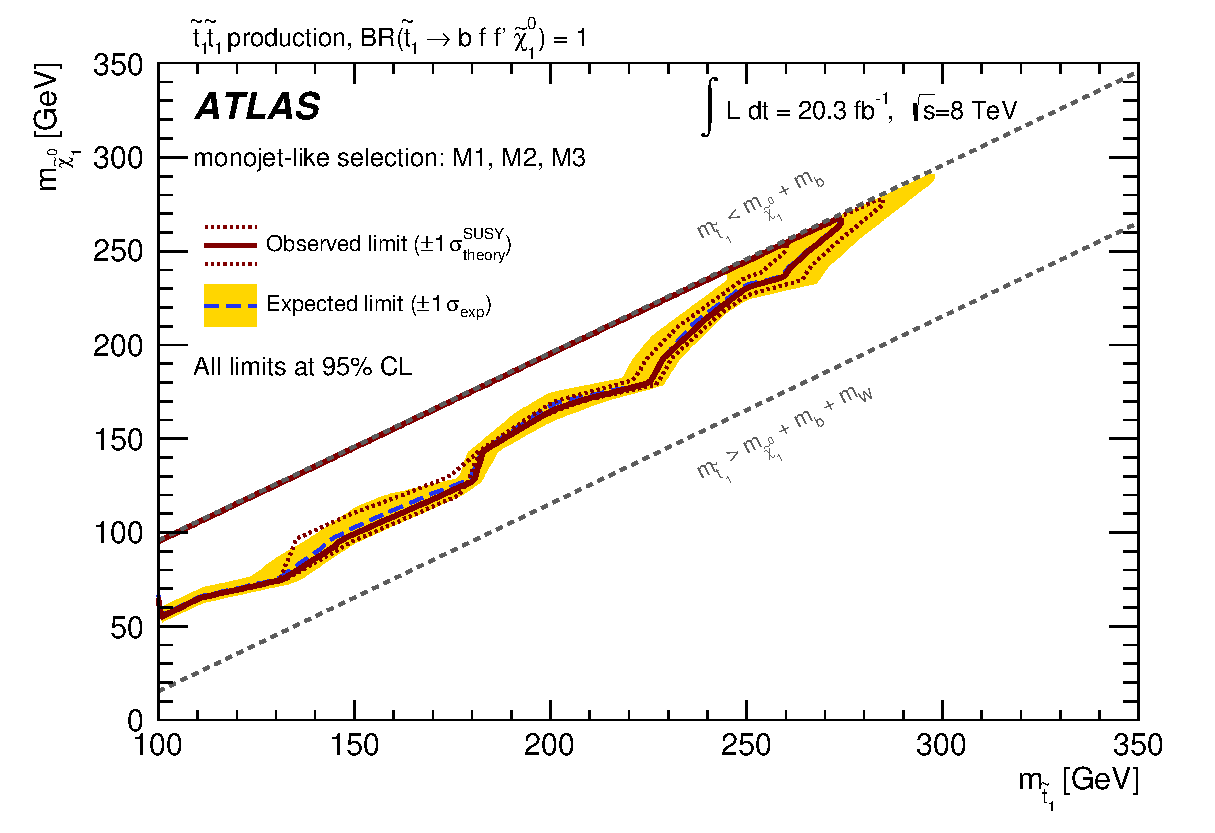
\includegraphics[width=0.795\textwidth]{Interpretations/Figures/limitPlotFourBody_Stop_combined_M1_M2_M3_.eps}
}
\end{center}
\caption[Exclusion plane at 95\% CL for stop pair production with $\stopfourbody$ as a function of the $m_{\stop}$ and $m_{\ninoone}$]{Exclusion plane at 95\% CL as a function of stop and neutralino masses for the decay channel $\stopfourbody$ (BR=100\%). The dotted lines around the observed limit indicate the range of observed limits corresponding to $\pm 1 \sigma$ variations on the NLO SUSY cross section predictions. The shaded area around the expected limit indicates the expected $\pm 1 \sigma$ ranges of limits in the absence of a signal. A band for $m_{\stopone} - m_{\ninoone}< \unit[2]{GeV}$ indicates the region in the phase space for which the stop can become long-lived \protect\cite{Aad:2014nra}.}
\label{fig:ExclusionStopToFourbody}
\end{figure}


\subsection{Mixed scenarios}

The exclusion limits shown in Figures \ref{fig:ExclusionStoptocharm} and \ref{fig:ExclusionStopToFourbody} are produced assuming a 100\% branching ratio to $\stoptocharm$ and $\stopfourbody$, respectively.
In the following, the monojet analysis is interpreted in terms of stop pair production, considering the stops decays $\stoptocharm$ or $\stopfourbody$, with different branching ratios, and assuming that $\text{BR}(\stoptocharm)$ + $\text{BR}(\stopfourbody)$ = 1.
For this purpose, new samples are generated, following the prescriptions detailed in Section~\ref{sec:MCSamples}, and assuming each stop to decay in a different final state.
The expected number of events for a model with a $\text{BR}(\stoptocharm) = \alpha$ can be computed with the following expression:

\begin{equation}
\begin{split}
N_{\alpha} &= \alpha^2 N_{\stopone\stopone \;\rightarrow \;c\ninoone \; c\ninoone} + 2\alpha(1-\alpha)N_{\stopone\stopone \;\rightarrow \;c\ninoone \; bff'\ninoone} \\
&+ (1-\alpha)^2 N_{\stopone\stopone \;\rightarrow \;bff'\ninoone \;bff'\ninoone},
\end{split}
\label{eq:MixedSamplesCombination}
\end{equation}

\noindent where $N_{\stopone\stopone \;\rightarrow \;c\ninoone \; c\ninoone}$, $N_{\stopone\stopone \;\rightarrow \;c\ninoone \; bff'\ninoone}$, and $N_{\stopone\stopone \;\rightarrow \;bff'\ninoone \;bff'\ninoone}$ are the number of events from the stop pair production assuming BR$(\stoptocharm)=1$, BR$(\stopfourbody)=1$, and $\text{BR}(\stoptocharm) = \text{BR}(\stopfourbody) = 0.5$, respectively.

Figure \ref{fig:ExclusionMixed} shows the 95\% CL upper cross section limits as a function of the stop mass and the branching fractions (red lines) for two different $\Delta m$ configurations.
These upper limits can be compared to the nominal $\stopone$ pair production cross section (blue line).

\begin{figure}[!t]
\begin{center}
\mbox{
\includegraphics[width=0.795\textwidth]{Interpretations/Figures/upperLimitXSectionBR_Stop_dM_10_M1_M2_M3.eps}
}
\mbox{
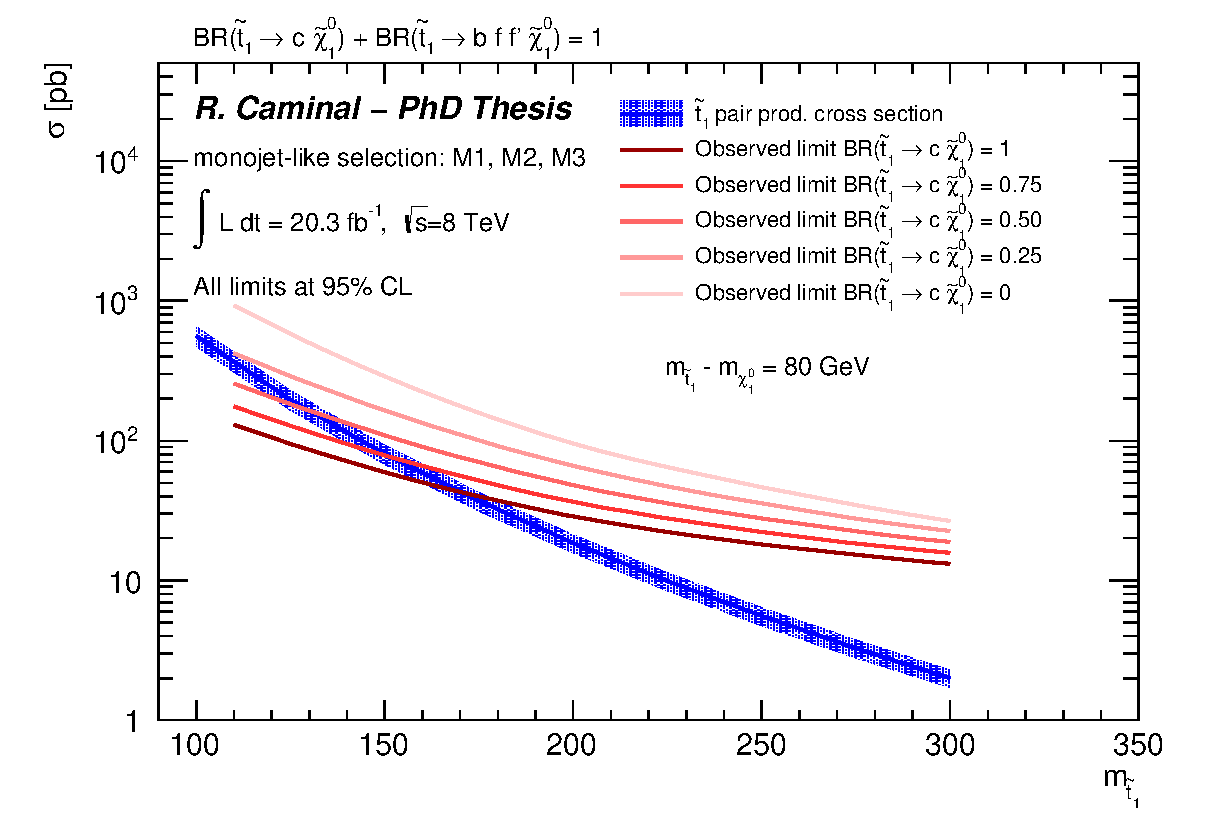
\includegraphics[width=0.795\textwidth]{Interpretations/Figures/upperLimitXSectionBR_Stop_dM_80_M1_M2_M3.eps}
}
\end{center}
\caption[Upper limits on the stop pair production cross section at 95\% CL as a function of $m_{\stopone}$ for different branching ratios.]{95\% CL upper cross section limits as a function of the stop mass (in red) compared to the $\stopone$ pair nominal cross section (in blue). $\Delta m = \unit[10]{GeV}$ and $\Delta m = \unit[80]{GeV}$ models are considered in the top and bottom figures respectively.}
\label{fig:ExclusionMixed}
\end{figure}

When $\Delta m = \unit[10]{GeV}$, the available phase space for the products of the stop decay is reduced, and thus the selection relies only on the production of an ISR jet.
The exclusion is independent on the branching ratio, when the stop and the neutralino are almost degenerated in mass.
Instead, when $\Delta m = \unit[80]{GeV}$ the Standard Model decay products of each stop are boosted enough to be reconstructed.
The $\stopfourbody$ decay of the stop is more affected by the jet multiplicity requirement and the lepton vetoes, than the $\stoptocharm$.
For this reason, less stringent limits on the mass of the stop can be set, as the branching ratio to $\stopfourbody$ increases.


\section{Direct sbottom pair production}
    \label{sec:DirectSbottomProduction}

In the case of bottom squark pair production, it is assumed a SUSY particle mass hierarchy such that the sbottom decays exclusively into a bottom quark and a neutralino, $\sbottomtob$.
Figure~\ref{fig:Diagrams3rdGen} (right) shows a Feynman diagram for this decay.
The expected signal for the direct sbottom pair is characterized by the presence of two energetic jets from the hadronization of the bottom quarks and large $\met$ from the two LSPs in the final state.
The monojet results are interpreted in terms of this search, $\sbottomtob$, in compressed scenarios.
The sbottom and the neutralino masses are almost degenerated, leading to two soft $b$-jets and an energetic ISR in the final state.

Signal regions M1 to M3 are used, and for each mass point the one with best expected $CL_s$ is chosen, as shown in Figure~\ref{fig:ExclusionSbottomtob} (top).
Figure \ref{fig:ExclusionSbottomtob} (bottom) shows the exclusion limits at 95\% CL for the $\sbottomtob$ model, as a function of the sbottom and neutralino masses.
The fact that the exclusion for very low or very high $\Delta m$ is better than for medium $\Delta m$ has to do with the acceptance, with the negotiation between mass and momentum investment for the neutralino, and the phase space available for extra radiation.
The cross section is independent of the $\Delta m$ for fixed sbottom masses, so the $CL_s$ values for the different mass configurations depend exclusively on acceptance and efficiency.
For all neutralino masses, the sbottoms are boosted by an initial-state radiation.
Scenarios with small $\Delta m$ (large neutralino mass), are characterized by soft $b$-jets (hardly ever identified) and little extra ISR/FSR.
As the mass of the neutralino decreases (medium $\Delta m$), the two $b$-jets are reconstructed and there is more phase space available for extra jet radiations.
Therefore, more events fail the jet veto selection and the sensitivity of the monojet analysis to this region of the phase space decreases.
For large $\Delta m$ configurations (low neutralino masses), the loss of sensitivity due to extra jet radiation is compensated by the increase in $\met$ due to the highly boosted neutralinos.

Sbottom masses below $\unit[180]{GeV}$ can be excluded for arbitrary neutralino masses.
In the case of sbottom and neutralino degenerated in mass, this analysis excludes sbottom masses up to $\unit[255]{GeV}$, thus expanding the exclusion limits set by other searches \cite{Aaltonen:2010dy,Abazov:2010wq,Aad:2013ija}.
For very low neutralino masses, the analysis also excludes sbottom masses up to $\unit[255]{GeV}$.


\begin{figure}[!ht]
\begin{center}
\mbox{
\includegraphics[width=0.795\textwidth]{Interpretations/Figures/limitPlotSbottom_Stop_combined_M1_M2_M3_BestRegion.eps}
}
\mbox{
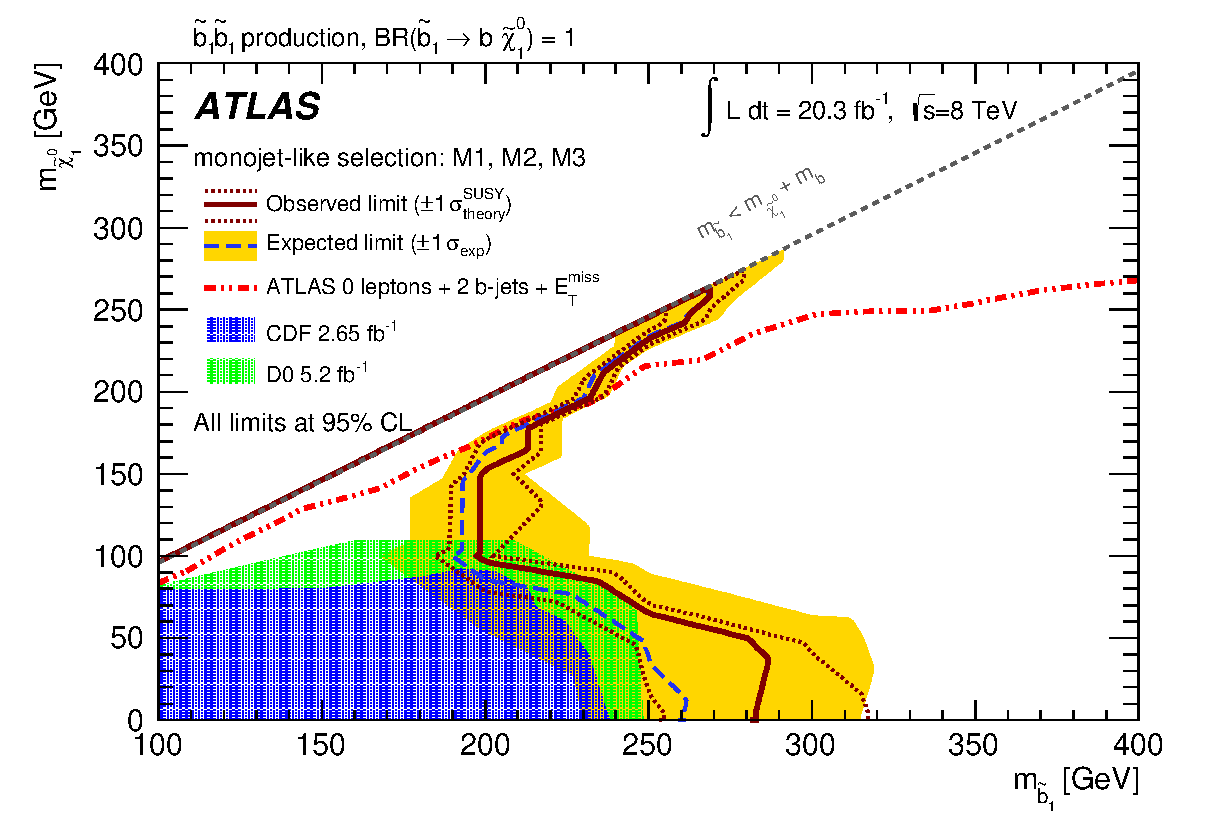
\includegraphics[width=0.795\textwidth]{Interpretations/Figures/limitPlotSbottom_Stop_combined_M1_M2_M3_.eps}
}
\end{center}
\caption[Exclusion plane at 95\% CL for sbottom pair production with $\sbottomtob$ as a function of the $m_{\sbottom}$ and $m_{\ninoone}$]{Exclusion plane at 95\% CL as a function of sbottom and neutralino masses for the decay channel $\sbottomtob$ (BR=100\%). The observed (red line) and expected (blue line) upper limits from this analysis are compared to previous results from CDF~\cite{Aaltonen:2010dy}, D0~\cite{Abazov:2010wq}, and ATLAS~\cite{Aad:2013ija}. For the latter, the area below the dashed-dotted line is excluded. The dotted lines around the observed limit indicate the range of observed limits corresponding to $\pm 1 \sigma$ variations on the NLO SUSY cross section predictions. The shaded area around the expected limit indicates the expected $\pm 1 \sigma$ ranges of limits in the absence of a signal. A band for $m_{\sbottomone} - m_{\ninoone}< \unit[2]{GeV}$  indicates the region in the phase space for which the sbottom can become long-lived. \protect\cite{Aad:2014nra}.}
\label{fig:ExclusionSbottomtob}
\end{figure}



%%%%%%%%%%%%%%%%%%%%%%%%%%%%%%%%%%%%%%%%%%%%%%%%%%%%%%%%%%%%%%%%%%%%%%%%%%%%%%%%%%%%%%%%%%%%%%%%%%%%%%%%%%%%%%%%%%%%%%%%%%%%%%%%%%%%%%%


\cleardoublepage
\chapter{Interpretations: inclusive squarks or gluinos}
    \label{chapter:SquarkGluinoProduction}

This chapter presents the interpretation of the monojet analysis in terms of models involving the direct production of inclusive squarks, or gluinos.
Only the signal regions M1 to M3 are considered, and the one giving the best expected exclusion is used for the results.


\section{Inclusive squark pair production}
    \label{sec:InclusiveSquarkProduction}

This section presents the interpretation of the analysis in terms of pair production of degenerated light-flavour squarks, with each squark decaying into a light quark and a neutralino (see Figure \ref{fig:DiagramsInclusiveProduction} left).
The MC samples for this model have been simulated with \madgraph{} and \pythia{}, using the PDF set CTEQ6L1.
The renormalization and factorization scales are set to the mass of the mean mass of the participating particles, $Q=(m_{\squark}+m_{\gluino})/2$.
The AUET2B tune has been used for the simulation of the underlying event, while the MLM matching scheme is used with up to one additional jet in the \madgraph{} matrix element.
More detailed information on these samples can be found in Ref.~\cite{Aad:2014wea}.
Different mass points have been generated for this process, in a grid with squark masses ranging between $\unit[87]{GeV}$ and $\unit[1225]{GeV}$, and neutralino masses between $\unit[0]{GeV}$ and those corresponding to a $\Delta m = m_{\squark} - m_{\ninoone}$ equal to $\unit[10]{GeV}$.
The signal cross sections are calculated to NLO in the strong coupling constant, adding the resummation of soft gluon emission at next-to-leading-logarithmic pQCD accuracy (NLO+NLL).

Experimental and theoretical systematic uncertainties for the different mass configurations have been computed, as explained in Section~\ref{sec:SysUncertaintiesSignal}.
Figure~\ref{fig:signalAcceptanceSquark} shows the impact of the scale variations on the signal acceptance for different squark masses as a function of $\Delta m$.
The uncertainties on the factorization and renormalization scales can be modeled as shown in Ref.~\cite{Aad:2014wea}.
The validity of this parametrization, shown in the figure by the dashed blue line, has been carefully checked for the monojet analysis, and is finally adopted.
In the case of the matching scale uncertainty, a flat 10\% is considered, based on the studies from Fig.~\ref{fig:signalAcceptanceSquark} (right).
Altogether, the systematic uncertainty on the acceptance for the signal is parametrized as:

\begin{equation}
\left(\frac{\Delta N}{N}\right)_{\text{signal}} = 0.15 \times e^{-{\Delta m / 250}} \oplus 0.20 \times e^{-{\Delta m / 250}} \oplus 0.1.
\label{eq:systematicAcceptanceSquark}
\end{equation}

\begin{figure}[t!]
\begin{center}
\includegraphics[width=0.32\textwidth]{Interpretations/Figures/signalUncert_mu_M1.eps}
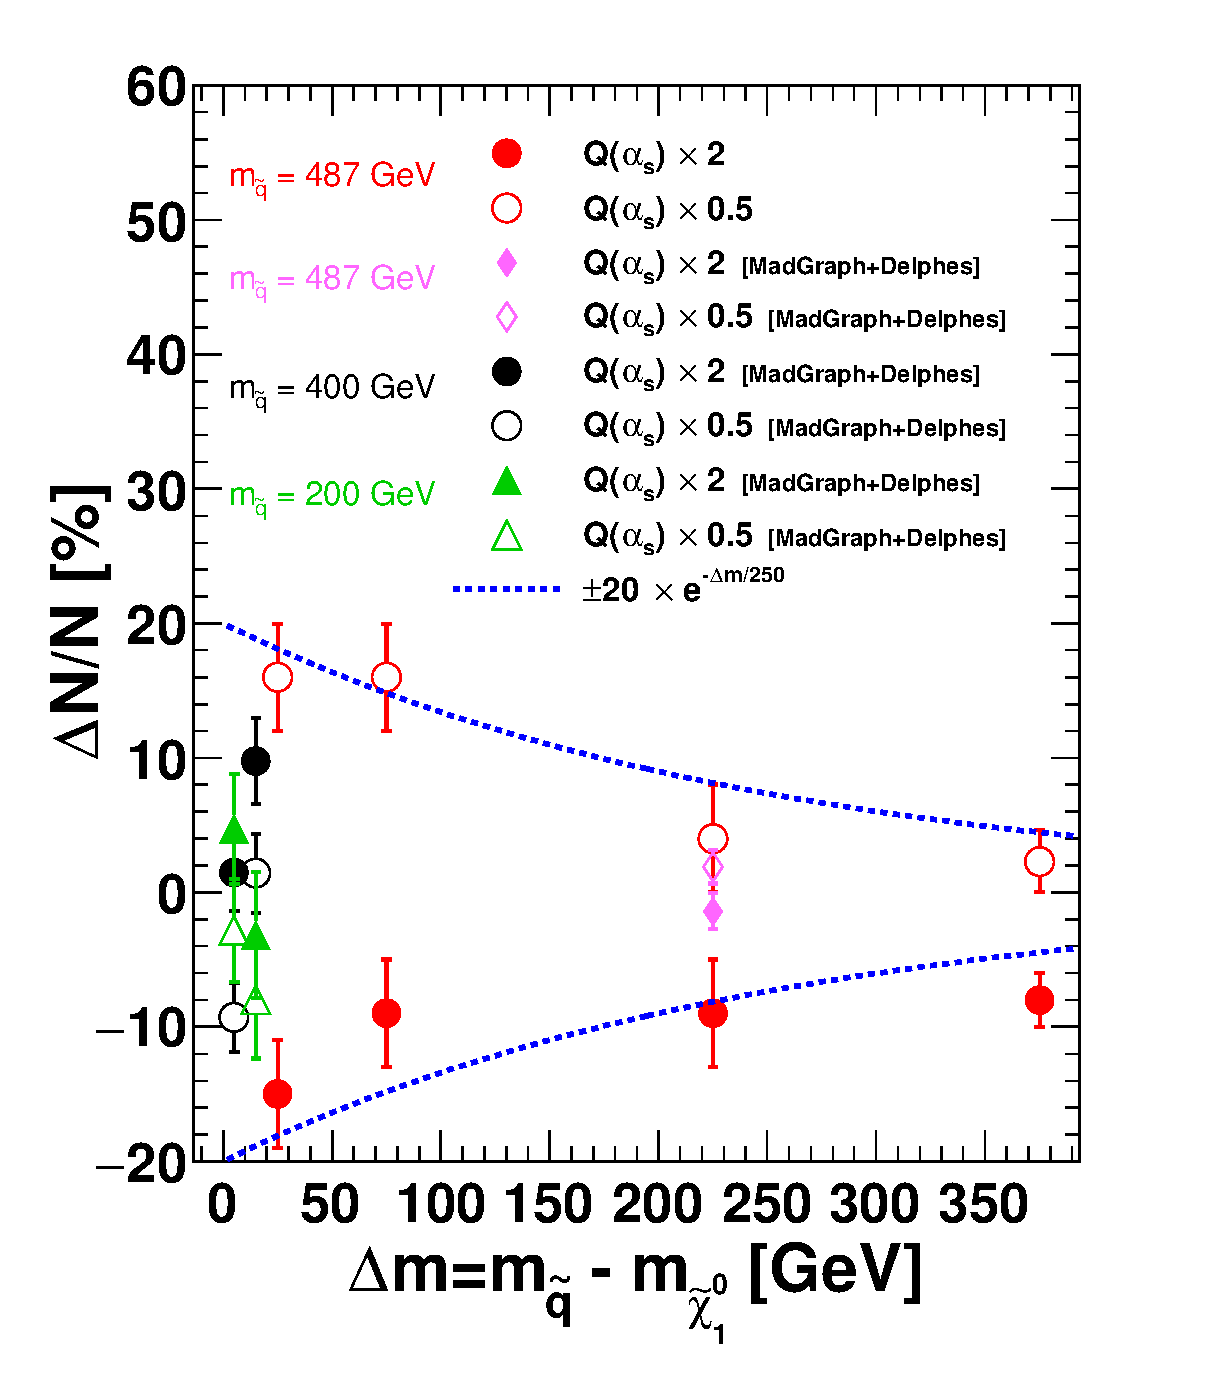
\includegraphics[width=0.32\textwidth]{Interpretations/Figures/signalUncert_Q_M1.eps}
\includegraphics[width=0.32\textwidth]{Interpretations/Figures/signalUncert_Matching_M1.eps}
\end{center}
\caption[Parametrization of the theoretical systematic uncertainties for the squark pair production when $\squarktoq$.]{The red points show the impact of (left) renormalization/factorization $\mu$, (center) $Q(\alpha _s)$ and (right) matching scales used in \madgraph{}+\pythia{} on the number of expected events $N$ for a simplified model with $\squark$ pair production (\squark$\rightarrow q+$\ninoone). The relative effect $\Delta N/N$ after proper normalization to the same total cross section is shown as a function of $\Delta m = m_{\tilde{q}} - m_{\tilde{\chi}_1^0}$. The dashed lines show the parameterization used to compute the uncertainties on the signal acceptance~\cite{Aad:2014wea}. The points in black and green show similar measurements in the monojet M1 signal region done with \madgraph{} samples for the low $\Delta m$ points used in the monojet-like analysis.}
\label{fig:signalAcceptanceSquark}
\end{figure}


\subsection{Exclusion Limits at 95\% CL}

The exclusion limits at 95\% CL for the first- and second-generation squark pair production are shown in Figure~\ref{fig:ExclusionSquarktoq}, as a function of the squark and neutralino masses.
The shape of the exclusion is related to the acceptance of the monojet analysis for each mass configuration, and follows the same arguments as for the sbottom pair production with $\sbottomtob$, shown in Section~\ref{sec:DirectSbottomProduction}.

Squark masses up to $\unit[320]{GeV}$ are excluded at 95\% CL for arbitrary neutralino masses.
For very compressed scenarios, the monojet analysis excludes squark masses up to $\unit[440]{GeV}$, thus extending the exclusion limits of the analysis in Ref.~\cite{Aad:2014wea} and shown in the figure.
Masses up to $\unit[660]{GeV}$ are also excluded for neutralino masses below 20~GeV.


\begin{figure}[!t]
  \begin{center}
    \mbox{
      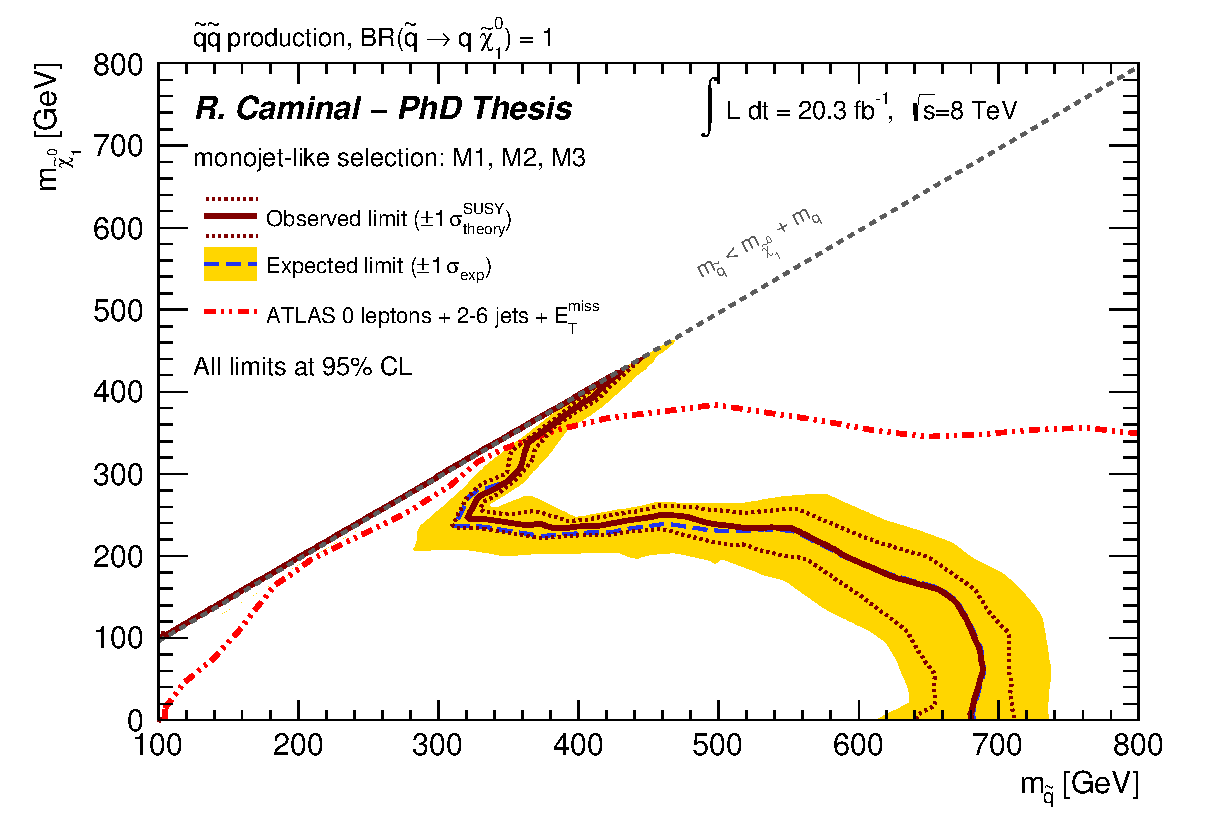
\includegraphics[width=0.795\textwidth]{Interpretations/Figures/limitPlotSquark_Stop_combined_M1_M2_M3_.eps}
    }
  \end{center}
  \caption[Exclusion plane at 95\% CL for sbottom pair production with $\squarktoq$ as a function of the $m_{\squark}$ and $m_{\ninoone}$]{Exclusion plane at 95\% CL as a function of the squark and neutralino masses for the $\squarktoq$ process. The dotted lines around the observed limit indicate the range of observed limits corresponding to the $\pm 1 \sigma$ variations on the cross section predictions. The shaded area around the expected limit indicates the expected $\pm 1 \sigma$ ranges of limits in the absence of a signal.
  The upper limits from this analysis are also compared to the previous results from ATLAS~\cite{Aad:2014wea}, shown in the figure with a dot-dashed red line.}
  \label{fig:ExclusionSquarktoq}
\end{figure}


\section{Gluino pair production}
    \label{sec:GluinoProduction}

Similarly, the results have been interpreted in terms of final states involving the production of pairs of gluinos.
Two different decay modes of the gluino have been considered.
First, the gluino is assumed to decay with 100\% branching fraction into a bottom quark and a virtual sbottom, which then decays into another bottom quark plus a neutralino, $\gluinotobb$.
In the second decay mode under consideration, the gluino decays exclusively to a gluon and a neutralino, $\gluinotog$, via a loop in which the interchange of a quark is involved.
The Feynman diagrams for both processes are shown in the middle and right panes of Figure~\ref{fig:DiagramsInclusiveProduction}.
The calculation of experimental and theoretical uncertainties follows the procedure explained in Section~\ref{sec:SysUncertaintiesSignal}.


\subsection{Gluino decaying to two $b$-quarks and a neutralino}

Samples for gluino pair production with $\gluinotobb$ have been simulated using \madgraph{} with one additional jet from matrix element and \pythia{-6} for the showering, following the same prescriptions as for the $\squarktoq$ simulated samples.
A grid of points with the gluino mass between $\unit[200]{GeV}$ to $\unit[1600]{GeV}$ and neutralino masses between $\unit[1]{GeV}$ and values corresponding to a $\Delta m = \unit[25]{GeV}$ has been produced.

The 95\% CL exclusion limits as a function of the gluino and neutralino masses are shown in Figure~\ref{fig:ExclusionGluinoGbb}.
The monojet analysis allows to expand the excluded parameter space in Ref.~\cite{TheATLAScollaboration:2013tha} towards compressed gluino and neutralino mass configurations.
Gluino masses up to $\unit[580]{GeV}$ can be excluded for low $\Delta m = m_{\gluino} - m_{\ninoone}$ values.
As the difference between the gluino and neutralino masses increases, the bottom quarks from the gluino decays are more boosted and the $b$-jets can be reconstructed.
Therefore, the analysis looses sensitivity to these configurations due to the jet veto requirement in the selections.
Gluino masses up to $\unit[420]{GeV}$ are excluded for very low neutralino masses.

\begin{figure}[!ht]
  \begin{center}
    \mbox{
      \includegraphics[width=0.795\textwidth]{Interpretations/Figures/limitPlotGluinoGbb_Stop_combined_M1_M2_M3_.eps}
    }
  \end{center}
  \caption[Exclusion plane at 95\% CL for gluino pair production with $\gluinotobb$ as a function of the $m_{\gluino}$ and $m_{\ninoone}$]{Exclusion plane at 95\% CL as a function of the gluino and neutralino masses for the $\gluinotobb$ process. The dotted lines around the observed limit indicate the range of observed limits corresponding to the $\pm 1 \sigma$ variations on the cross section predictions. The shaded area around the expected limit indicates the expected $\pm 1 \sigma$ ranges of limits in the absence of a signal.
  The upper limits from this analysis are also compared to the previous results from ATLAS~\cite{TheATLAScollaboration:2013tha}, shown in the figure with a dot-dashed red line.}
  \label{fig:ExclusionGluinoGbb}
\end{figure}


\subsection{Gluino decaying to a gluon and a neutralino}

Finally, a second grid for gluino pair production with $\gluinotog$ has been produced with the same prescriptions as the $\gluinotobb$ samples.
The production consists of several samples with gluino masses between $\unit[150]{GeV}$ and $\unit[1500]{GeV}$, and neutralino masses between $\unit[0]{GeV}$ and values corresponding to $\Delta m = \unit[50]{GeV}$.
Figure \ref{fig:ExclusionGluinoGg} shows the 95\% CL exclusion plane as a function of the gluino and neutralino masses.
Gluinos with masses up to 600~GeV are excluded at 95\% CL for the very compressed scenario.
For massless neutralinos, gluino masses up to 850~GeV can be excluded.

\begin{figure}[!ht]
  \begin{center}
    \mbox{
      \includegraphics[width=0.795\textwidth]{Interpretations/Figures/limitPlotGluinoGg_Stop_combined_M1_M2_M3_.eps}
    }
  \end{center}
  \caption[Exclusion plane at 95\% CL for gluino pair production with $\gluinotog$ as a function of the $m_{\gluino}$ and $m_{\ninoone}$]{Exclusion plane at 95\% CL as a function of the gluino and neutralino masses for the $\gluinotog$ process. The dotted lines around the observed limit indicate the range of observed limits corresponding to the $\pm 1 \sigma$ variations on the cross section predictions. The shaded area around the expected limit indicates the expected $\pm 1 \sigma$ ranges of limits in the absence of a signal.}
  \label{fig:ExclusionGluinoGg}
\end{figure}






%%%%%%%%%%%%%%%%%%%%%%%%%%%%%%%%%%%%%%%%%%%%%%%%%%%%%%%%%%%%%%%%%%%%%%%%%%%%%%%%%%%%%%%%%%%%%%%%%%%%%%%%%%%%%%%%%%%%%%%%%%%%%%%%%%%%%%%


\cleardoublepage
\chapter{Interpretations: Dark Matter related}

This chapter presents interpretations of the monojet analysis in terms of models involving the direct production of potential Dark Matter candidates.
This includes models based on effective theories, simplified models involving the pair production of Weakly Interacting Massive Particles, or the production of gravitinos in Gauge Mediated SUSY breaking scenarios.
Sensitivity studies of the monojet analysis to models involving the direct production of charginos or neutralinos are also collected in Appendix~\ref{sec:CharginoNeutralinoProduction}.

%------------------
%--- Section for the WIMPs, wrongly included first as an appendix!!!
%------------------
\section{WIMPs pair production}
    \label{sec:WIMPsProduction}

In this section, the results of the monojet analysis are converted into limits on the pair production of WIMPs. 
Samples for several models based on an effective theory (D5, D8 and D9, see Table~\ref{tab:WIMPsEffectiveOperators}) corresponding to the process $\wimpwimp$ have been generated.
They are implemented using LO matrix elements in \madgraph{}.
The WIMP pair production plus one or two additional partons from ISR/FSR is considered.
For each operator, a sample is generated requiring at least one parton with $\pt>\unit[80]{GeV}$, and another sample is generated with at least one parton with a minimum $\pt$ of 300~GeV.
The latter samples are needed to populate those signal regions with $\met$ requirements larger than 350~GeV.
Only initial states of the four lightest quarks are considered, assuming equal coupling strengths for all quark flavors to the WIMPs.
The generated events are interfaced to \pythia{} for the parton showering and hadronization.
The MLM prescription is used for matching the matrix element calculations to the parton shower evolution.
The PDF set CTEQ6L1 is used for the event simulation, and the renormalization and factorization scales are set to the geometric average of $m_{\chi}^2 + \pt^2$ for the two WIMPs, being $m_{\chi}$ is the mass of the WIMP.
Events with WIMP masses between $\unit[10]{GeV}$ and $\unit[1.3]{TeV}$ are simulated for the different effective operators considered.

To study the transition between the effective field theory and a physical renormalizable model for Dirac fermion WIMPs coupling to SM particles via a new mediator particle $Z'$, a simplified model is generated with \madgraph{}.
For each WIMP mass, mediator particle masses $M_{\text{med}}$ between $\unit[50]{GeV}$ and $\unit[13]{TeV}$ are considered, for two different mediator particle width each ($\Gamma_{\text{med}} = M_{\text{med}}/3$ and $\Gamma_{\text{med}} = M_{\text{med}}/8\pi$).
  
For each effective model, the limits are extracted from the signal region M3, since it has the best expected sensitivity.
This is translated into corresponding 90\% CL limits\footnote{The limits are extracted at 90\% CL instead of 95\% CL, in order for them to be compared to direct dark matter search experiments.} on the suppression scale $M^{\ast}$ as a function of $m_{\chi}$.
To derive the lower limits in $M^{\ast}$, the $CL_s$ approach described in Section~\ref{sec:ComputationOfLimits} is used.
    
The systematic uncertainties for these models are computed as described in Chapter~\ref{chapter:Interpretations}.
Experimental uncertainties on jets and $\met$ scale and resolution, lepton efficiency, and luminosity translate into a 5\% to 3\% uncertainty on the signal yields for D5 and D8 models for a WIMP masses between 50~GeV and 1.3~TeV.
For the model D9, the experimental uncertainty varies from 1.5\% to 4\% for the same WIMP mass range.
The theoretical uncertainties include: the uncertainty on the renormalization, factorization scales; the uncertainty on the matrix element to parton shower matching scales; the uncertainty on the modeling of the ISF/FSR and the uncertainty on the PDFs.
These uncertainties translate to an effect between 3\% to 8\% in the signal yield, depending on the operator and the WIMP mass.
    
The 90\% CL limits on $M^{\ast}$ for the operators D5 (vector), D8 (axial-vector) and D9 (tensor) are reported in Table~\ref{tab:WIMPsEffective_limit_mstar} and shown in Figure~\ref{fig:WIMPsEffectiveMstar}, down to WIMP masses of 10~GeV.
These limits are extrapolated even further to smaller $m_{\chi}$ values, since for such low-mass WIMPs there is a negligible change in the fiducial cross section and kinematic distributions.

%--- \ref{tab:WIMPsEffective_limit_mstar}
\begin{sidewaystable}[h!]
\centering
\begin{tabular}{c|cc|cc|cc}
\hline\hline
\multirow{2}{*}{{\bf $\mathbf{m_\chi}$ [GeV]}} & \multicolumn{2}{c|}{\bf $\mathbf{M^*}$ D5 (vector)} & \multicolumn{2}{c|}{\bf $\mathbf{M^*}$ D8 (axial-vector)} & \multicolumn{2}{c}{\bf $\mathbf{M^*}$ D9 (tensor)}\\ 
\cline{2-7}
           & {\bf Obs. [GeV]} & {\bf Exp. [GeV]} & {\bf Obs. [GeV]} & {\bf Exp. [GeV]} & {\bf Obs. [GeV]} & {\bf Exp. [GeV]}\\ 
\hline
    1      &    990 &   992 &   971 &   973 &   1672    &   1677    \\
    10     &    990 &   992 &   971 &   973 &   1672    &   1677    \\
    50     &    990 &   992 &   971 &   973 &   1715    &   1719    \\
    100 &   979 &   982 &   948 &   950 &   1613    &   1618    \\
    200 &   957 &   960 &   893 &   893 &   1541    &   1545    \\
    400 &   896 &   899 &   760 &   763 &   1294    &   1297    \\
    700 &   706 &   708 &   544 &   545 &   922 &   923 \\
    1000    &   507 &   509 &   367 &   369 &   634 &   636 \\
    1300    &   344 &   345 &   229     &   230     &   430 &   431     \\
    \hline\hline
    \end{tabular}
    \caption[The 90\% CL observed and expected limits on $M^*$ as a function of the WIMP mass $m_\chi$ for different interaction models.]{The 90\% CL observed and expected limits on $M^*$ as a function of the WIMP mass $m_\chi$ for D5 (vector), D8 (axial-vector) and D9 (tensor) interaction models.}
    \label{tab:WIMPsEffective_limit_mstar}
    \end{sidewaystable}



The effective theories used are based on the assumption that a new mediator particle couples SM particles to pairs of WIMPs, and that the mass of the mediator is much larger than the scale of the interaction.
If this is the case, the mediator cannot be produced directly in the collisions, and therefore it can be integrated out by the effective formalism.
However, this assumption is not always correct at the LHC, where the momentum transfer can reach the TeV energies.
For a given operator, one possible validity criterion would be that the momentum transferred in the hard interaction, $Q_{\text{tr}}$ is below the mediator mass, $M_{\text{med}}$, defined as $M_{\text{med}} = \sqrt{g_{q} g_{\chi}} M^{\ast}$, where $g_{q}$ and $g_{\chi}$ are the couplings of the mediator to the SM particles and the WIMPs, respectively.
Figure~\ref{fig:WIMPsEffectiveMstar} also shows the 90\% CL upper limit on $M^{\ast}$ when this ``truncation'' criteria ($Q<M_{\text{med}}$) is imposed, assuming $\sqrt{g_{q} g_{\chi}} = 1$.
The truncated limits fulfill the respective validity criteria wherever the lines are drawn in the figure.
For D5 (D9) for example, the criterion is fulfilled for WIMP masses up to 100~GeV (200~GeV).
No attempt is made to consider different couplings than $\sqrt{g_{q} g_{\chi}} = 1$ in these effective models.
The limits on $M^{\ast}$ for the truncated effective models are also quoted in Table~\ref{tab:WIMPsEffective_limit_mstar_trunc}.
The thermal relic lines are also included from Ref.~\cite{Goodman:2010ku} to this figure, corresponding to a coupling, set by $M^{\ast}$, of WIMPs to quarks such that WIMPs have the correct relic abundance as measured by the WMAP satelite~\cite{Larson:2010gs}, in the absense of any other interaction, apart from the one considered.

%--- \ref{tab:WIMPsEffective_limit_mstar_trunc}
\begin{table}[ht!]
   \centering
\begin{tabular}{ccc}
\hline\hline
{\bf $\mathbf{m_{\chi}}$ [GeV]} & {\bf $\mathbf{M^*}$ [GeV] D5 (vector)} & {\bf $\mathbf{M^*}$ [GeV] D9 (tensor)} \\ 
\hline
1	   &	600	&		-	      \\
10	   &	650	&		1600   	\\
25	   &	650	&		-         \\
50	   &	600	&		1650   	\\
100	   &	550	&		1550   	\\
200	   &	-   &		1450   	\\
\hline\hline
\end{tabular}
\caption{90\% CL Observed limit on $M^*$ for D5 and D9 models, with truncation of the events with $\sqrt{\hat{s}}>M^*$.}
\label{tab:WIMPsEffective_limit_mstar_trunc}
\end{table}


\begin{figure}[!t] 
   \centering
   \mbox{
   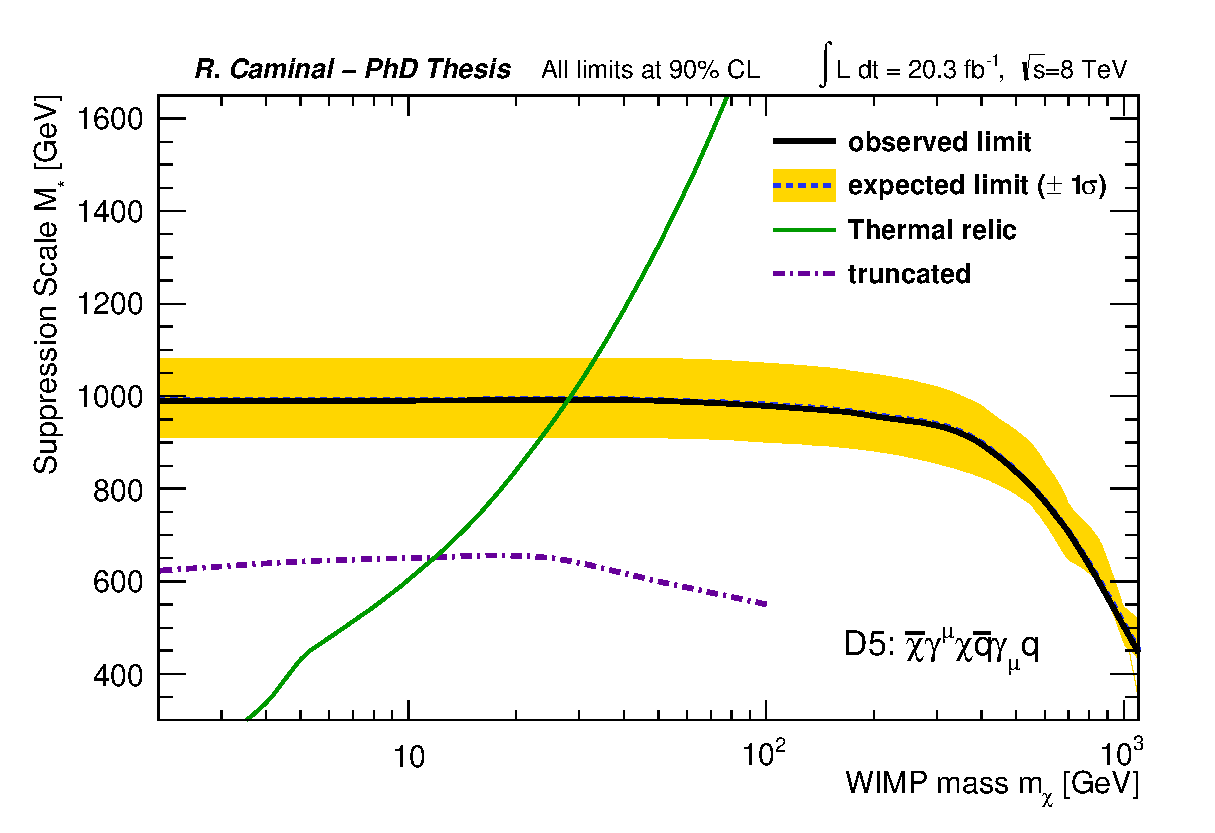
\includegraphics[width=0.495\textwidth]{Interpretations/Figures/WIMPmStar_D5.eps} 
   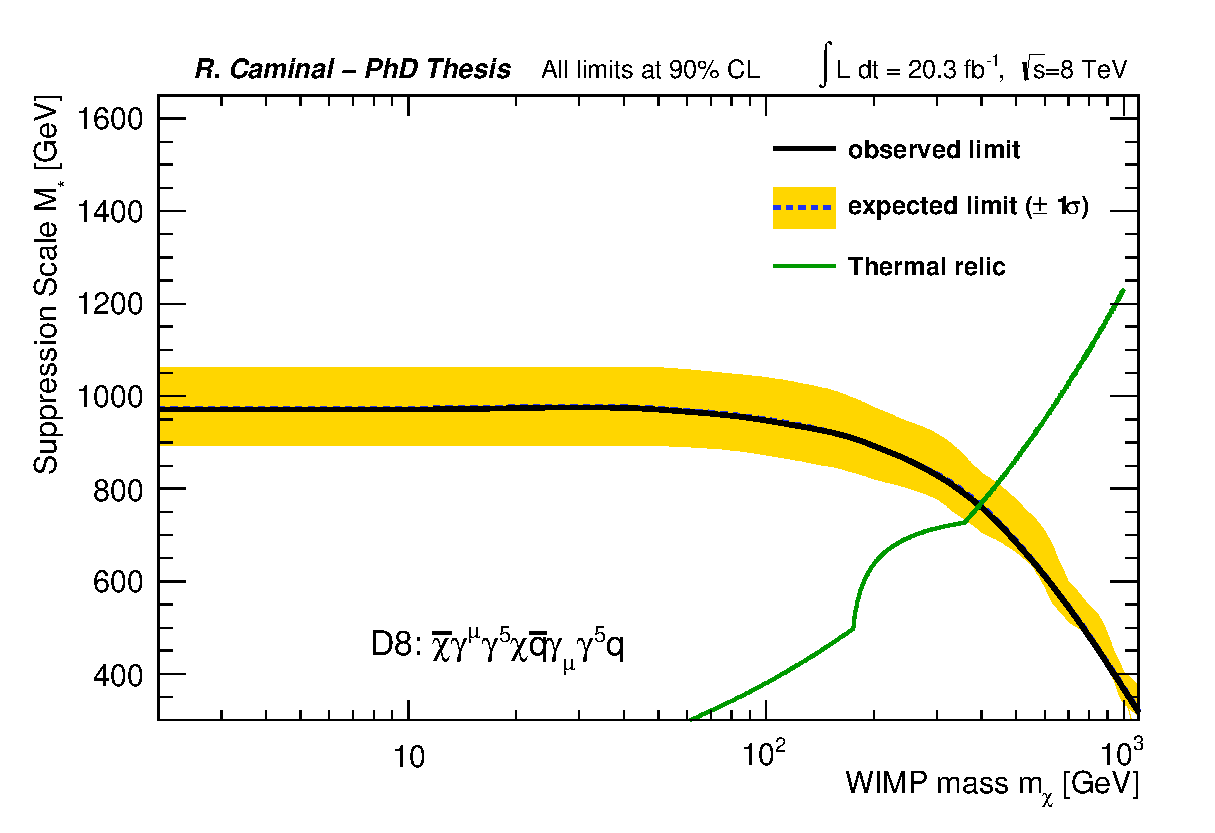
\includegraphics[width=0.495\textwidth]{Interpretations/Figures/WIMPmStar_D8.eps} 
   }
   \mbox{
   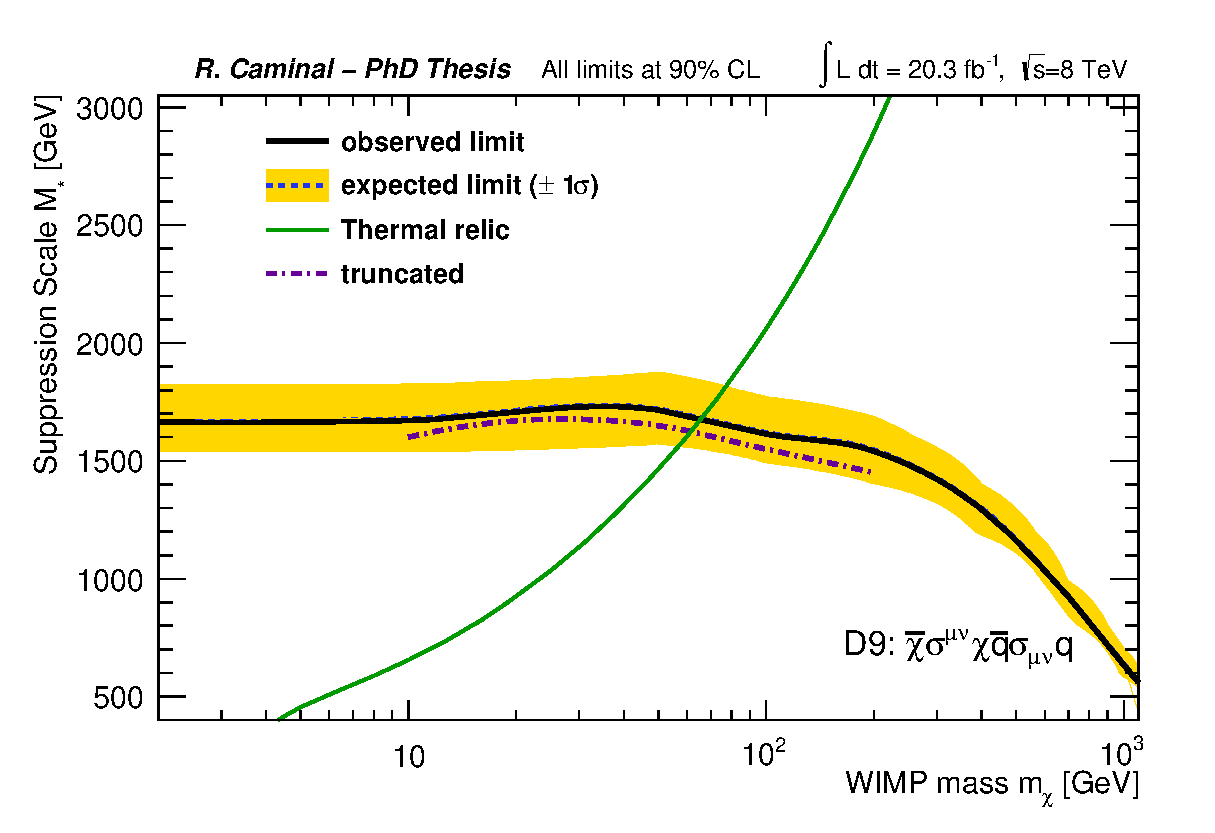
\includegraphics[width=0.495\textwidth]{Interpretations/Figures/WIMPmStar_D9.eps} 
   }
   \caption[Observed and expected 90\% CL limits on $M^*$ as a function of the WIMP mass $m_\chi$ for different operators in the selection M3.]{Expected and observed 90\% CL limits on $M^{\ast}$ as a function of the WIMP mass $m_\chi$ for an integrated luminosity of 20.3~\ifb for the D5 (vector), D8 (axial-vector) and D9 (tensor) operators in the M3 signal region. The Expected and observed limits are shown as dashed blue and solid black lines, respectively.
     The $\pm 1\sigma$ error band in yellow around the expected limit is due to the acceptance uncertainties (both experimental and theoretical). The rising green lines are the $M^{\ast}$ values at which WIMPs of the given mass result in the relic density as measured by WMAP~\cite{Larson:2010gs}, assuming annihilation in the early universe proceeded exclusively via the given operator.
     The thermal relic line for D8 has a bump feature at the top quark mass where the annihilation channel to top quarks opens.
     The purple dot-dashed  line is the 95\% CL observed limit on $M^{\ast}$ imposing a validity criterion with a coupling strength of 1.}
   \label{fig:WIMPsEffectiveMstar}
\end{figure}

A way to avoid the validity issues of the effective theories is to use a simplified model which includes a mediator explicitly.
Here as an example, a vector-like $Z'$ boson is considered, corresponding to the D5 operator in the effective theory framework, of a given mass, $M_{\text{med}}$, and width, $\Gamma_{\text{med}}$.
With this approach, the product of the coupling constants of the $Z'$ can be constrained.
Figure~\ref{fig:WIMPsSimplifiedCouplingLimit} shows the 90\% CL limits on $\sqrt{g_{q}g_{\chi}}$ as a function of $M_{\text{med}}$ for different values of the WIMP mass and the width of the mediator.
Couplings above 1 and 1.5 are excluded for WIMP masses between 25~GeV and 400~GeV, respectively, for mediator masses between 25~GeV and around 1~TeV.
For higher mediator masses, the limits on the couplings have higher values.
In particular, for mediator masses around 10~TeV, the couplings enter the non-perturbative regime and the theory is not anymore valid, for any WIMP mass and mediator width configuration.

\begin{figure}[!t]
  \begin{center}
    \mbox{
      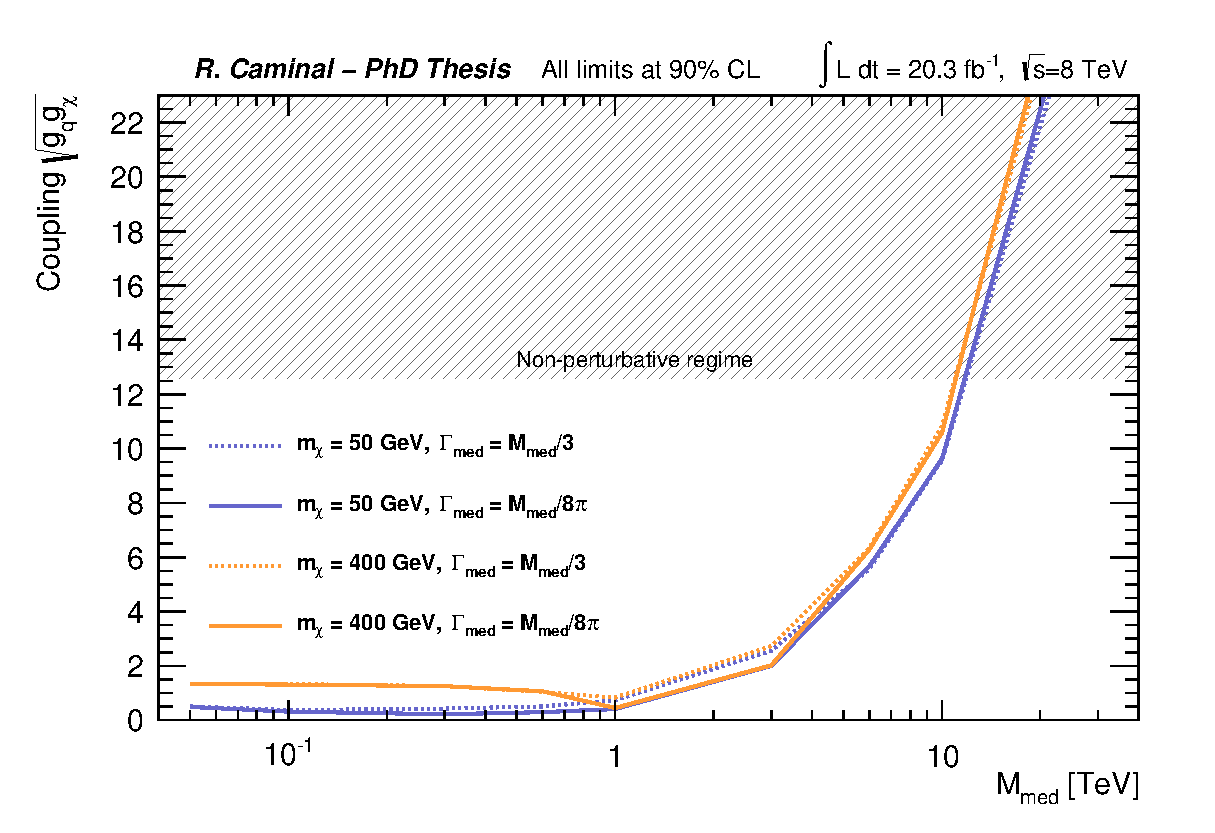
\includegraphics[width=0.795\textwidth]{Interpretations/Figures/WIMPsimplified_MmedCoupling.eps}
    }
  \end{center}
  \caption[Observed 90\% CL limits on the product of the coupling constants as a function of the mediator mass, assuming a $Z'$-like simplified model.]{Observed 90\% CL limits on the product of the coupling constants, $\sqrt{g_q g_\chi}$, as a function of the mediator mass, $M_\text{med}$, assuming a $Z'$-like simplified model and a DM mass of 50~GeV and 400~GeV. The width of the mediator is varied between $M_\text{med}/3$ and $M_\text{med}/8\pi$.}
  \label{fig:WIMPsSimplifiedCouplingLimit}
\end{figure}

These limits can be translated into 90\% CL limits on $M^{\ast}$ as a function of $M_{\text{med}}$.
Figure~\ref{fig:WIMPsSimplifiedMstarLimit} demonstrates how for a given mediator particle mass and two values of the width, the real value of the mass suppression scale would compare to the $M^{\ast}$ derived assuming a contact interaction (shown as dashed line in the figure).
This contact interaction regime is reached by values of the $M_{\text{med}}$ larger than 5~TeV.
In the $\unit[700]{GeV} < M_\text{med} < \unit[5]{TeV}$ the mediator would be produced resonantly, and therefore the actual $M^{\ast}$ value is higher than in the contact interaction regime.
For lower mediator masses, the limit on $M^{\ast}$ is very low, since the WIMP would be heavier than the mediator, and the WIMP pair production via this mediator would be kinematically suppressed.
In this region, the contact interaction limits would be optimistic and overestimate the actual $M^{\ast}$ values.

\begin{figure}[!t]
  \begin{center}
    \mbox{
      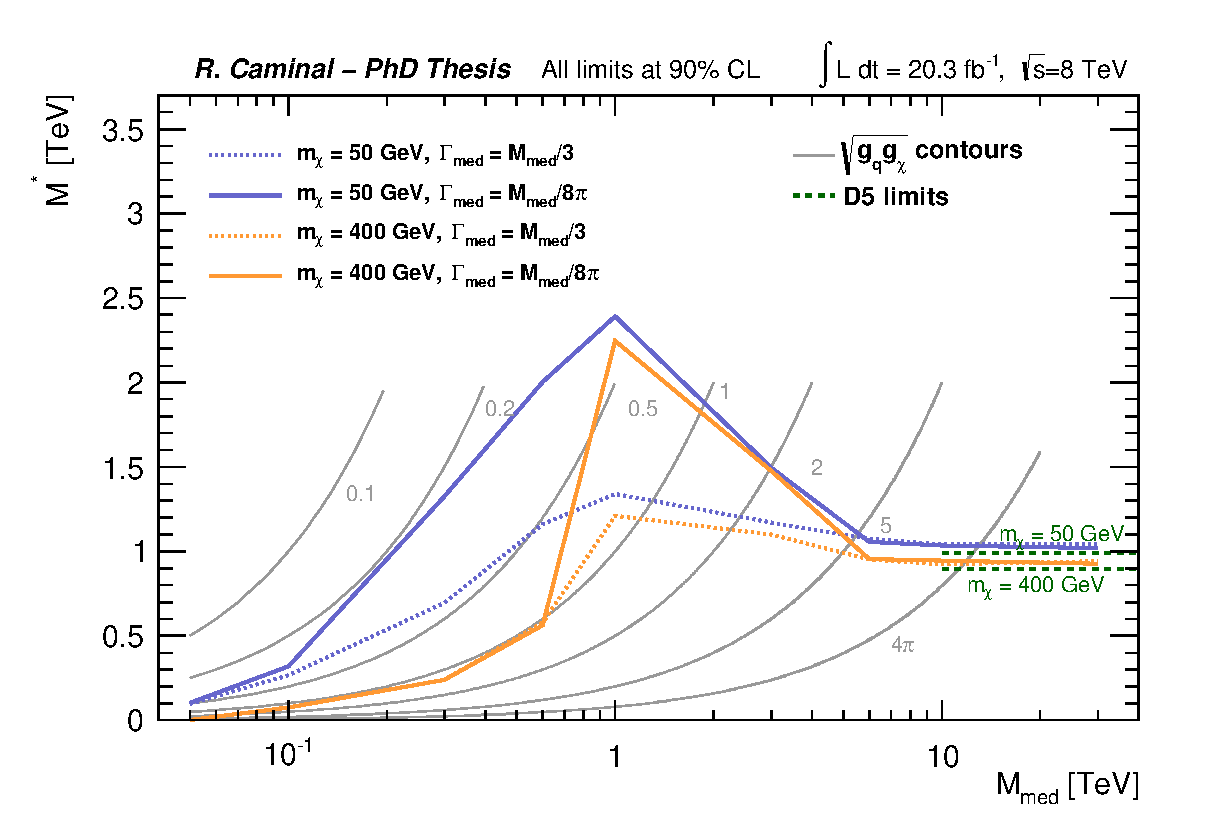
\includegraphics[width=0.795\textwidth]{Interpretations/Figures/WIMPsimplified_MstarMmed_vector.eps}
    }
  \end{center}
  \caption[Observed limits on $M^{\ast}$ as a function of the mediator mass assuming a $Z'$-like simplified model.]{Observed limits on $M^{\ast}$ as a function of the mediator mass, $M_\text{med}$, assuming a $Z'$-like simplified model and a DM mass of 50~GeV and 400~GeV.
  The width of the mediator is varied between $M_\text{med}/3$ and $M_\text{med}/8\pi$.
  The corresponding limits of the effective model D5 are shown as dashed lines.
  Contour lines indicating a range of values of the product of the coupling constants, $\sqrt{g_q g_\chi}$, are also shown.}
  \label{fig:WIMPsSimplifiedMstarLimit}
\end{figure}

In the effective operator approach, the bounds on $M^{\ast}$ for a given $m_{\chi}$ can be converted to bounds on WIMP-nucleon scattering cross section, $\sigma_{\chi N}$, probed by direct DM experiments, using the transformation equations \ref{eq:WIMP-Nucleon}:

\begin{equation}
\begin{split}
\sigma^{D5}_{\chi N} &= 1.38 \times \unit[10^{-37}]{cm^2} \times \left(\frac{\mu_{\chi}}{\unit[1]{GeV}}\right)^2\left(\frac{\unit[300]{GeV}}{M^{\ast}}\right)^4 \\
\sigma^{D8}_{\chi N} &= 4.70 \times \unit[10^{-40}]{cm^2} \times \left(\frac{\mu_{\chi}}{\unit[1]{GeV}}\right)^2\left(\frac{\unit[300]{GeV}}{M^{\ast}}\right)^4 \\
\sigma^{D9}_{\chi N} &= 4.70 \times \unit[10^{-40}]{cm^2} \times \left(\frac{\mu_{\chi}}{\unit[1]{GeV}}\right)^2\left(\frac{\unit[300]{GeV}}{M^{\ast}}\right)^4. \\
\end{split}
\label{eq:WIMP-Nucleon_2}
\end{equation}

These bounds describe the scattering of WIMPs from nucleons at a very low momentum transfer, of the order of the keV.
Depending on the type of interaction, contributions to spin-dependent and spin-independent WIMP-nucleon interactions are expected.
The 90\% CL lower limits on the WIMP-nucleon scattering cross section are shown in Figure~\ref{fig:WIMPsNucleonXSection}.
Under the assumption made by the effective approach, these limits are relevant in the low DM mass region, and remain important in the full $m_{\chi}$ range covered.
Cross sections above $\unit[2.7\times10^{-40}]{cm^{2}}$ ($\unit[7.0\times10^{-38}]{cm^{2}}$) are excluded for WIMP masses of 1~GeV (1.3~TeV), respectively.
The spin-dependent limits in this figure are based on D8 and D9, where for D8 the limits have been calculated with the D5 acceptances, since they are identical, together with the D8 production cross section.
Both limits are significantly stronger than those from direct-detection experiments.
For D8, cross sections above $\unit[1.0\times10^{-41}]{cm^{2}}$ ($\unit[1.2\times10^{-38}]{cm^{2}}$) are excluded at 90\% CL for WIMP masses of 1~GeV (1.3~TeV), respectively, while for D9, cross sections above $\unit[1.1\times10^{-42}]{cm^{2}}$ ($\unit[9.8\times10^{-40}]{cm^{2}}$) are excluded in the same WIMP mass range.
The limits on the non-truncated and truncated $\sigma_{\chi N}$ are also shown in Tables~\ref{tab:WIMPsEffective_limit_sigma} and~\ref{tab:WIMPsEffective_limit_sigma_truncated}, respectively.

%--- \ref{tab:WIMPsEffective_limit_sigma}
\begin{sidewaystable}[h!]
   \centering
\begin{tabular}{c|cc|cc|cc}
\hline\hline
\multirow{2}{*}{{\bf $\mathbf{m_\chi}$ [GeV]}} & \multicolumn{2}{c|}{{\bf $\mathbf{\sigma_{\chi N}}$(D5)}} & \multicolumn{2}{c|}{{\bf $\mathbf{\sigma_{\chi N}}$(D8)}} & \multicolumn{2}{c}{{\bf $\mathbf{\sigma_{\chi N}}$(D9)}}\\ 
\cline{2-7}
       & {\bf Obs. [GeV]} & {\bf Exp. [cm$^2$]} & {\bf Obs. [cm$^2$]} & {\bf Exp. [cm$^2$]} & {\bf Obs. [cm$^2$]} & {\bf Exp. [cm$^2$]}\\ 
\hline
1	   &	2.73$\times 10^{-40}$	&	2.71$\times 10^{-40}$	&	1.00$\times 10^{-41}$	&	9.95$\times 10^{-42}$	&	1.14$\times 10^{-42}$	&	1.13$\times 10^{-42}$	\\
10	   &	8.56$\times 10^{-40}$	&	8.49$\times 10^{-40}$	&	3.15$\times 10^{-41}$	&	3.13$\times 10^{-41}$	&	3.58$\times 10^{-42}$	&	3.54$\times 10^{-42}$	\\
50	   &	9.87$\times 10^{-40}$	&	9.79$\times 10^{-40}$	&	3.63$\times 10^{-41}$	&	3.60$\times 10^{-41}$	&	3.73$\times 10^{-42}$	&	3.70$\times 10^{-42}$	\\
100	&	1.05$\times 10^{-39}$	&	1.04$\times 10^{-39}$	&	4.07$\times 10^{-41}$	&	4.04$\times 10^{-41}$	&	4.86$\times 10^{-42}$	&	4.80$\times 10^{-42}$	\\
200	&	1.16$\times 10^{-39}$	&	1.15$\times 10^{-39}$	&	5.22$\times 10^{-41}$	&	5.17$\times 10^{-41}$	&	5.89$\times 10^{-42}$	&	5.83$\times 10^{-42}$	\\
400	&	1.52$\times 10^{-39}$	&	1.50$\times 10^{-39}$	&	1.00$\times 10^{-40}$	&	9.84$\times 10^{-41}$	&	1.19$\times 10^{-41}$	&	1.18$\times 10^{-41}$	\\
700	&	3.95$\times 10^{-39}$	&	3.91$\times 10^{-39}$	&	3.81$\times 10^{-40}$	&	3.79$\times 10^{-40}$	&	4.63$\times 10^{-41}$	&	4.61$\times 10^{-41}$	\\
1000	&	1.49$\times 10^{-38}$	&	1.46$\times 10^{-38}$	&	1.84$\times 10^{-39}$	&	1.80$\times 10^{-39}$	&	2.07$\times 10^{-40}$	&	2.05$\times 10^{-40}$	\\
1300	&	7.02$\times 10^{-38}$	&	6.94$\times 10^{-38}$	&	1.22$\times 10^{-38}$ 	&	1.20$\times 10^{-38}$ 	&	9.79$\times 10^{-40}$	&	9.70$\times 10^{-40}$ 	\\
\hline\hline
\end{tabular}
\caption[The 90\% CL observed and expected limits on the WIMP-Nucleon scattering cross-section $\sigma_{\chi N}$ as a function of the WIMP mass $m_\chi$ for different interaction models.]{The 90\% CL observed and expected limits on the WIMP-Nucleon scattering cross-section $\sigma_{\chi N}$ as a function of the WIMP mass $m_\chi$ for D5 (vector), D8 (axial-vector) and D9 (tensor) interaction models.}
\label{tab:WIMPsEffective_limit_sigma}
\end{sidewaystable}



%--- \ref{tab:WIMPsEffective_limit_sigma_truncated}
\begin{table}[ht!]
   \centering
\begin{tabular}{ccc}
\hline\hline
$\mathbf{m_{\chi}}$ \textbf{[GeV]}               & {\bf $\mathbf{\sigma_{\chi N}}$(D5)} & {\bf $\mathbf{\sigma_{\chi N}}$(D9)} \\ 
\hline
1	   &	2.02$\times 10^{-39}$	&		-        	            \\
10	   &	4.61$\times 10^{-39}$	&		4.27$\times 10^{-42}$	\\
25	   &	5.12$\times 10^{-39}$	&		-        	            \\
50	   &	7.31$\times 10^{-39}$	&		4.36$\times 10^{-42}$	\\
100	   &	1.06$\times 10^{-38}$	&		5.70$\times 10^{-42}$	\\
200	   &	-                    	&		7.51$\times 10^{-42}$	\\
\hline\hline
\end{tabular}
\caption[The 90\% CL Observed limit on WIMP-nucleon cross section for D5 and D9 models, with truncation of the events with $\sqrt{\hat{s}}>M^*$.]{The 90\% CL Observed limit on WIMP-nucleon cross section, $\sigma_{\chi-N}$, for D5 and D9 models, with truncation of the events with $\sqrt{\hat{s}}>M^*$.}
\label{tab:WIMPsEffective_limit_sigma_truncated}
\end{table}


\begin{figure}[ht] 
   \centering
   \mbox{
     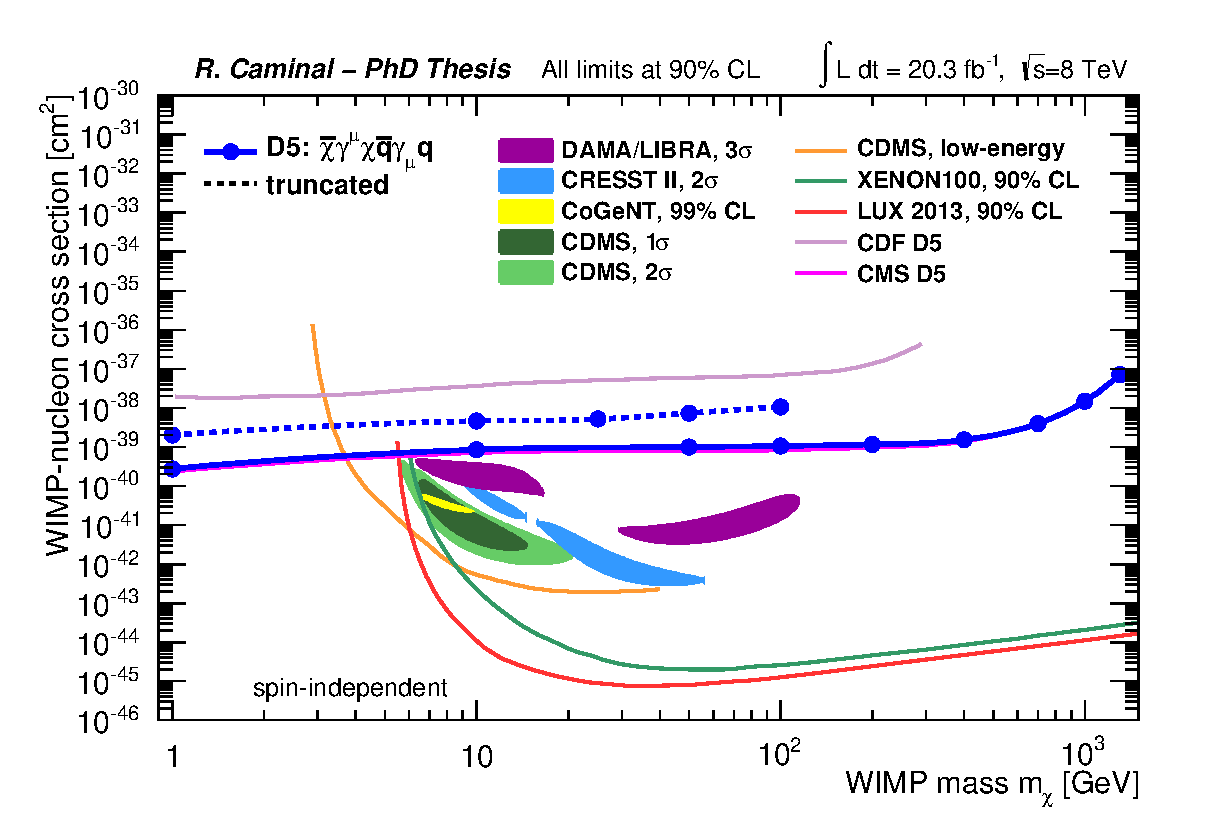
\includegraphics[width=0.795\textwidth]{Interpretations/Figures/WIMPnucleonXsection_spinIndependent.eps} 
   }
   \mbox{
     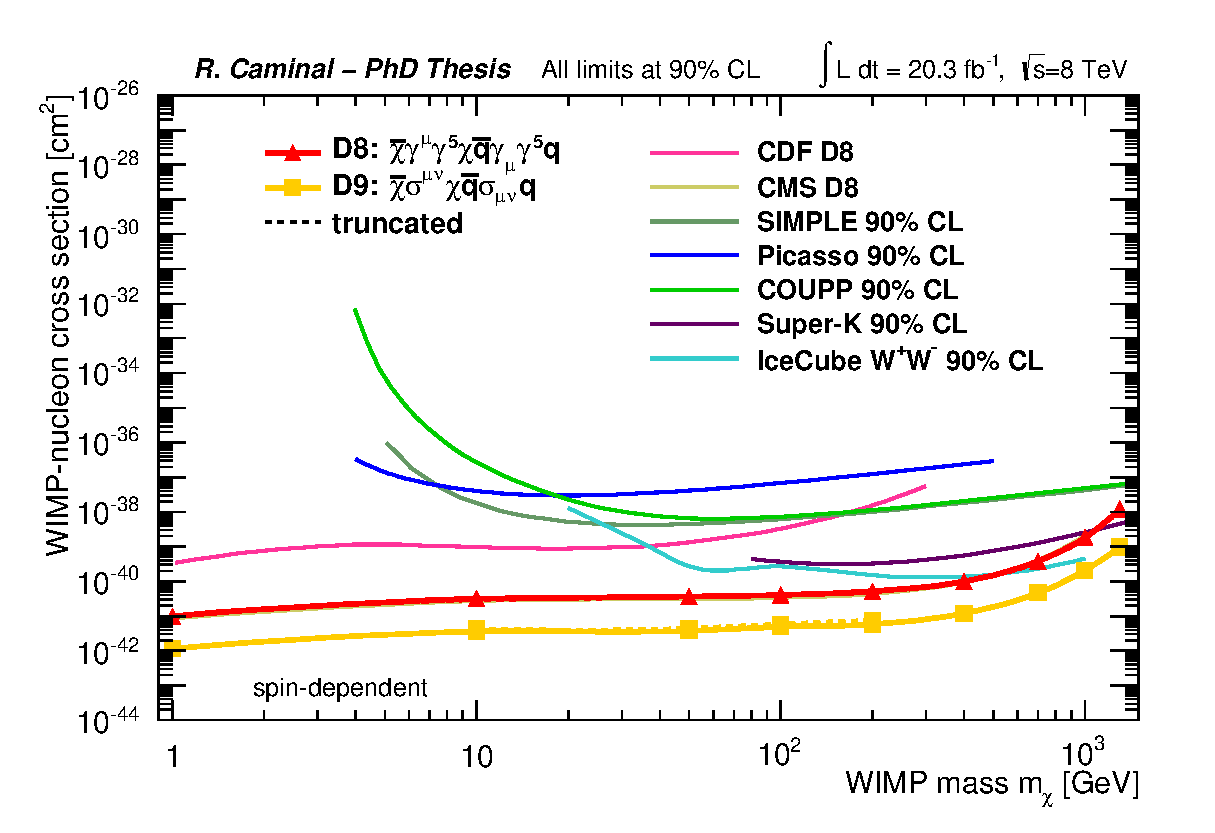
\includegraphics[width=0.795\textwidth]{Interpretations/Figures/WIMPnucleonXsection_spinDependent.eps} 
   }
\caption[90\% CL lower limits on spin-independent and spin-dependent the WIMP-nucleon scattering cross section.]{The 90\% CL lower limits on spin-independent (top) and spin-dependent (bottom) WIMP-nucleon scattering cross section for different masses of $\chi$ in M3 signal region. 
 Results from direct detection experiments for the spin-independent~\cite{Angloher:2011uu,Akerib:2013tjd,Agnese:2013rvf,Agnese:2014aze,Aalseth:2014jpa,Bernabei:2008yi,Bernabei:2010mq,Aprile:2012nq,Aprile:2013doa} and spin-dependent~\cite{Archambault:2012pm,Desai:2004pq,Abbasi:2009uz,Behnke:2010xt,Felizardo:2011uw} cross section, and the CMS (untruncated) limits~\cite{CMS:rwa} are also shown for comparison.}
\label{fig:WIMPsNucleonXSection}
\end{figure}

%--- 90 % confidence level limits (to be compared to the 95% CL of the monojet exotics!!!)
%--- Only the simplified models have no theoretical uncertainties on the acceptance.

%------------------
%------------------
%------------------


\section{Gravitino production in GMSB}
    \label{sec:GravitinoProduction}

In Gauge Mediated SUSY breaking scenarios, the gravitino mass gives direct access to the scale of the SUSY breaking, and can potentially contribute to the total amount of Dark Matter in the Universe.
In this section, the monojet results are interpreted in the context of gravitino production in association with a squark or a gluino in the final state.
Figure~\ref{fig:DiagramsGravitinoGMSB} shows some of the Feynman diagrams for this process.
A simplified SUSY model is used for which the squark or the gluino decays to a gravitino, and a quark or a gluon in the final state (see Figure~\ref{fig:DiagramsVertexGravitinoGMSB}), thus leading to a monojet signature.

Monte Carlo samples corresponding to gravitino production in association with a gluino or a squark in the final state, $\pp\rightarrow\squark\gravino+X$ and $\pp\rightarrow\gluino\gravino+X$ are generated at LO using \madgraph{}, interfaced with \pythia{} for the showering.
The ATLAS detector simulation is provided by the ATLAS fast simulation, while the PDF set used is CTEQ6L1.
The renormalization and factorization scales are set to the average of the mass of the final state particles involved in the hard interaction $(m_{\gravino} + m_{\squark , \gluino})/2 \simeq m_{\squark , \gluino}/2$.
A grid with different mass configurations has been generated with $m_{\squark, \gluino}$ from $\unit[50]{GeV}$ to $\unit[2.6]{TeV}$ and $m_{\squark}/m_{\gluino} = 0.25, 0.5, 1, 2, 4$, and a gravitino mass $m_{\gravino} = \unit[5 \times 10^{-4}]{eV}$.
Both experimental and theoretical systematic uncertainties for the different mass configurations are computed as for the previous models discussed in Section~\ref{sec:SysUncertaintiesSignal}.
Experimental uncertainties result into a 4.6\% to 2.9\% effect on the signal yield in M3, and a 16\% to 3\% effect in M6 for squark and gluino masses of 200~GeV and 2.4~TeV, respectively.
The theoretical uncertainties on the acceptance introduce a variation in the signal yield of about 15\%, while the theoretical uncertainties on the cross section contribute altogether to a 24\% to 55\% on the signal yield for different squark and gluino masses.


\subsection{Exclusion Limits at 95\% CL}

In this case, the 95\% CL limits on the visible cross section of the monojet analysis shown in Table~\ref{tab:modelIndependent} are used to extract the limits on the gravitino mass as a function of the masses of the squark or the gluinos.
The best sensitivity to the gravitino production is obtained for the selections M3, M5 and M6, and depends on the squark and gluino mass configuration.
Figure~\ref{fig:modelIndependentGravitino} shows, for the signal region M5, the fiducial cross section as a function of the squark and gluino mass, for different gravitino masses.
For comparison, the model independent limits from Table~\ref{tab:modelIndependent} are shown.
The intersection between the model independent limit and the signal fiducial cross section determines the exclusion in terms of the parameters of the model.
The following limits are calculated:

\begin{figure}[!ht]
\begin{center}
\mbox{
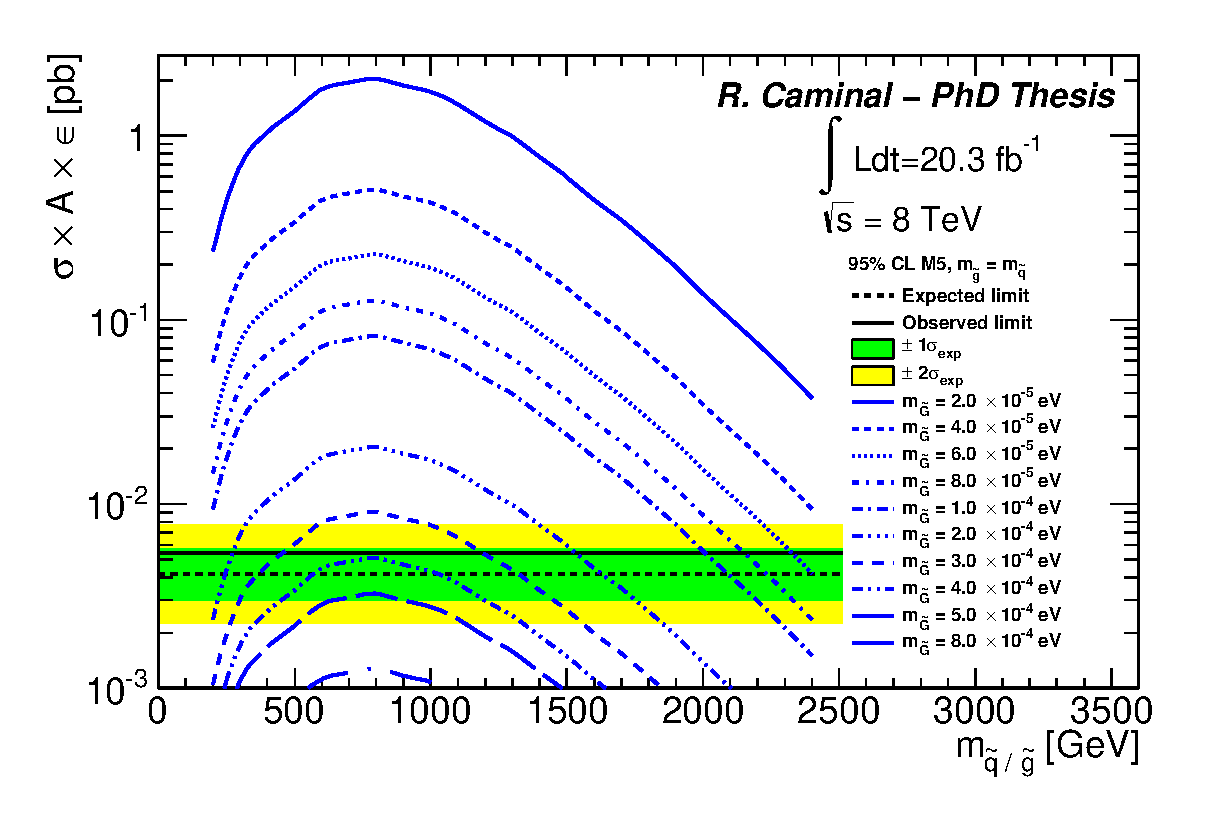
\includegraphics[width=0.995\textwidth]{Interpretations/Figures/ModelIndependentGravitino_mGVariable_Stop_A9.eps}
}
\end{center}
\caption[Fiducial cross section for the $\gravino + \squark / \gluino$ production as a function of the squark/gluino mass for degenerate squark and gluinos in the signal region M5.]{Fiducial cross section, $\sigma \times A \times \epsilon$, for the $\gravino + \squark / \gluino$ production as a function of the squark/gluino mass for degenerate squark and gluinos in the signal region M5. Different values of the gravitino mass are considered and the predictions are compared to the model independent limits (see Table \ref{tab:modelIndependent}).}
\label{fig:modelIndependentGravitino}
\end{figure}

\begin{itemize}
\item{Observed:}
intersection between the observed model independent limit and the signal visible cross section.
\item{Observed $- 1\sigma_{\text{total}}^{\text{signal}}$:}
intersection between the observed model independent limit and the signal visible cross section $- 1\sigma$ of the total uncertainty on the signal.
The total uncertainty is computed by summing in quadrature the experimental uncertainties and both the theoretical uncertainties on the acceptance and on the cross section.
\item{Observed $- 1\sigma_{\text{exp}}^{\text{signal}}$:}
intersection between the observed limit and the signal visible cross section $-1\sigma$ of the experimental uncertainty on the signal together with the effects of the modeling uncertainty on the signal acceptance (no cross section uncertainty is considered in this case).
\item{Expected:}
intersection between the expected model independent limit and the signal visible cross section.
\item{Expected $\pm 1\sigma$ or $\pm 2\sigma$:}
intersection between the signal visible cross section and the expected limit with $\pm 1\sigma$ or $\pm 2\sigma$ experimental uncertainty on the Standard Model background.
\end{itemize}

This approach does not take into account the correlations between the signal and the background uncertainties.
The $CL_s$ computation for each of the mass configurations in the grid would require a huge computational power, thus making the analysis very time consuming.
Tests performed for several cases showed that the exclusions using the model independent limits or using the $CL_s$ method return compatible, almost identical, results.

Figure~\ref{fig:GravitinoMassExclusion_mqmg} shows the 95\% CL limits on the gravitino mass, $m_{\gravino}$, for equal squark and gluino masses.
Gravitino masses below $3.5\times10^{-4}$~eV, $3\times10^{-4}$~eV and $2\times10^{-4}$~eV are excluded at 95\% CL for squark/gluino masses of 500~GeV, 1~TeV and 1.5~TeV.
For very high squark/gluino masses the narrow-width approximation (NWA) employed is violated since the partial width for the gluino and squark to decay into a gravitino and a parton becomes more than 25\% of its mass.
In this case, other decay channels for the gluino and squarks should be considered, leading to a different final state.
Figures~\ref{fig:GravitinoMassExclusion_xmqmg} and~\ref{fig:GravitinoMassExclusion_mqxmg} show the limits on the gravitino mass, for $m_{\gluino} = 2\times m_{\squark}$ and $m_{\gluino} = 4\times m_{\squark}$; and $m_{\gluino} = m_{\squark}/2$ and $m_{\gluino} = m_{\squark}/4$, respectively.
In this case, lower bounds on gravitino mass in the range between $5\times10^{-4}$ and $5\times10^{-5}$ are set depending on the squark and gluino masses.

\begin{figure}[!ht]
\begin{center}
\mbox{
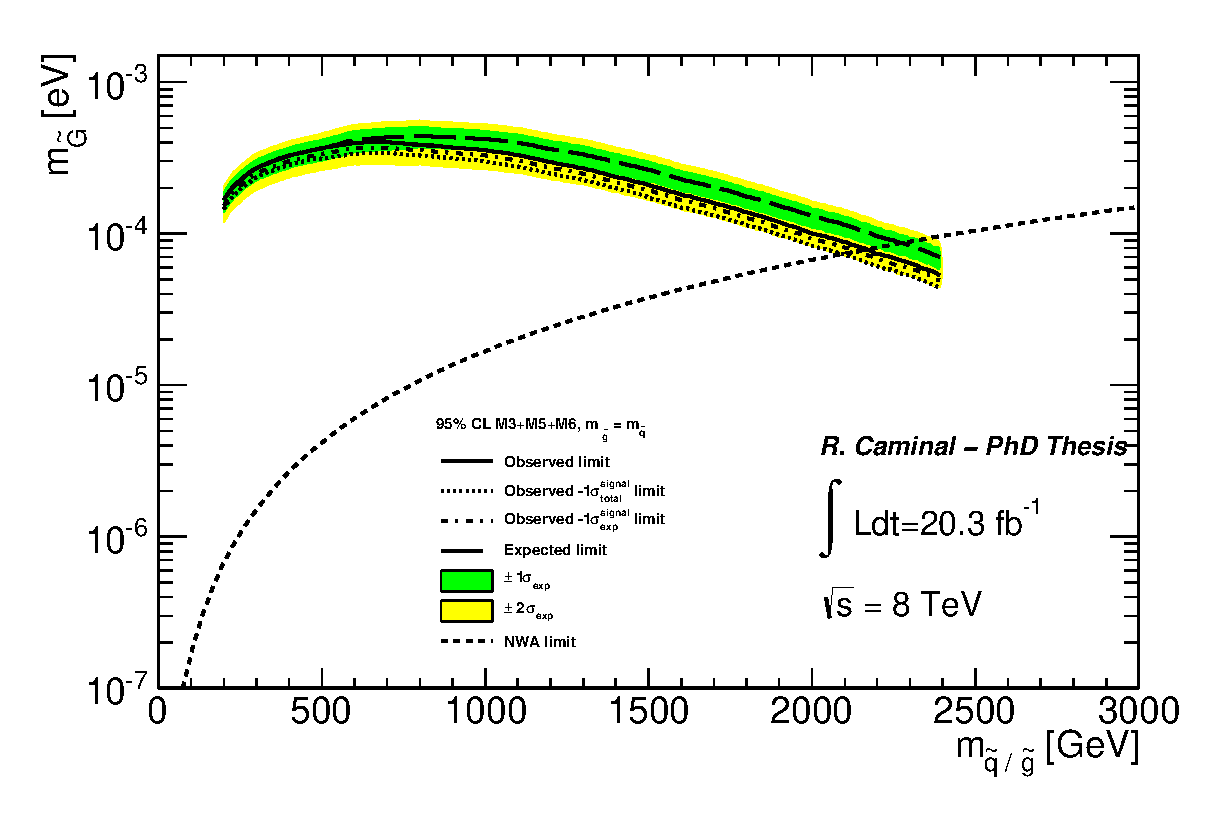
\includegraphics[width=0.795\textwidth]{Interpretations/Figures/ModelIndependentGravitino_combined_mGLimit_Stop_A4_A9_A10.eps}
}
\end{center}
\caption[95\% CL lower limits on the gravitino mass as a function of the squark mass for equal squark and neutralino masses.]{Observed (solid line) and expected (dashed line) 95\% CL lower limits on the gravitino mass as a function of the squark mass for equal squark and neutralino masses. The dotted line indicates the impact on the observed limit of the $\pm1\sigma$ LO theoretical uncertainty. The shaded bands around the expected line indicate the expected $\pm1\sigma$ and $\pm2\sigma$ ranges of limits. 
  The region above the black dotted line defines the validity of the narrow-width approximation (NWA) for which the decay width is smaller than 25\% of the squark/gluino mass.}
\label{fig:GravitinoMassExclusion_mqmg}
\end{figure}

\begin{figure}[!ht]
\begin{center}
\mbox{
\includegraphics[width=0.795\textwidth]{Interpretations/Figures/ModelIndependentGravitino_combined_mGLimit_Stop_A4_A9_A102mqmg.eps}
}
\mbox{
\includegraphics[width=0.795\textwidth]{Interpretations/Figures/ModelIndependentGravitino_combined_mGLimit_Stop_A4_A9_A104mqmg.eps}
}
\end{center}
\caption[95\% CL lower limits on the gravitino mass as a function of the squark mass for $m_{\gluino} = 2 \times m_{\squark}$ and $m_{\gluino} = 4 \times m_{\squark}$.]{Observed (solid line) and expected (dashed line) 95\% CL lower limits on the gravitino mass as a function of the squark mass for $m_{\gluino} = 2 \times m_{\squark}$ (top) and $m_{\gluino} = 4 \times m_{\squark}$ (bottom). The dotted line indicates the impact on the observed limit of the $\pm1\sigma$ LO theoretical uncertainty. The shaded bands around the expected line indicate the expected $\pm1\sigma$ and $\pm2\sigma$ ranges of limits. 
  The region above the black dotted line defines the validity of the narrow-width approximation (NWA) for which the decay width is smaller than 25\% of the squark/gluino mass.}
\label{fig:GravitinoMassExclusion_xmqmg}
\end{figure}

\begin{figure}[!ht]
\begin{center}
\mbox{
\includegraphics[width=0.795\textwidth]{Interpretations/Figures/ModelIndependentGravitino_combined_mGLimit_Stop_A4_A9_A10mq2mg.eps}
}
\mbox{
\includegraphics[width=0.795\textwidth]{Interpretations/Figures/ModelIndependentGravitino_combined_mGLimit_Stop_A4_A9_A10mq4mg.eps}
}
\end{center}
\caption[95\% CL lower limits on the gravitino mass as a function of the squark mass for $m_{\gluino} = 1/2 \times m_{\squark}$ and $m_{\gluino} = 1/4 \times m_{\squark}$.]{Observed (solid line) and expected (dashed line) 95\% CL lower limits on the gravitino mass as a function of the squark mass for $m_{\gluino} = 1/2 \times m_{\squark}$ (top) and $m_{\gluino} = 1/4 \times m_{\squark}$ (bottom). The dotted line indicates the impact on the observed limit of the $\pm1\sigma$ LO theoretical uncertainty. The shaded bands around the expected line indicate the expected $\pm1\sigma$ and $\pm2\sigma$ ranges of limits. 
  The region above the black dotted line defines the validity of the narrow-width approximation (NWA) for which the decay width is smaller than 25\% of the squark/gluino mass.}
\label{fig:GravitinoMassExclusion_mqxmg}
\end{figure}

The limits on the gravitino mass shown in Figures~\ref{fig:GravitinoMassExclusion_mqmg} to~\ref{fig:GravitinoMassExclusion_mqxmg} can be translated into 95\% CL upper limits on the breaking scale of SUSY, $\sqrt{\langle F \rangle}$.
These limits are shown in Figures~\ref{fig:GravitinoSqrtFExclusion_mqmg} to~\ref{fig:GravitinoSqrtFExclusion_mqxmg}, for the different squark and gluino mass configurations.
Values of the $\sqrt{\langle F \rangle}$ below 1~TeV can be excluded for squark/gluino masses of 1~TeV.

\begin{figure}[!ht]
\begin{center}
\mbox{
\includegraphics[width=0.795\textwidth]{Interpretations/Figures/ModelIndependentGravitino_combined_sqrtFLimit_Stop_A4_A9_A10.eps}
}
\end{center}
\caption[95\% CL lower limits on the SUSY breaking scale $F$ as a function of the squark mass for equal squark and neutralino masses.]{Observed (solid line) and expected (dashed line) 95\% CL lower limits on the SUSY breaking scale $F$ as a function of the squark mass for equal squark and neutralino masses. The dotted line indicates the impact on the observed limit of the $\pm1\sigma$ LO theoretical uncertainty. The shaded bands around the expected line indicate the expected $\pm1\sigma$ and $\pm2\sigma$ ranges of limits. 
  The region above the black dotted line defines the validity of the narrow-width approximation (NWA) for which the decay width is smaller than 25\% of the squark/gluino mass.}
\label{fig:GravitinoSqrtFExclusion_mqmg}
\end{figure}

\begin{figure}[!ht]
\begin{center}
\mbox{
\includegraphics[width=0.795\textwidth]{Interpretations/Figures/ModelIndependentGravitino_combined_sqrtFLimit_Stop_A4_A9_A102mqmg.eps}
}
\mbox{
\includegraphics[width=0.795\textwidth]{Interpretations/Figures/ModelIndependentGravitino_combined_sqrtFLimit_Stop_A4_A9_A104mqmg.eps}
}
\end{center}
\caption[95\% CL lower limits on the SUSY breaking scale $F$ as a function of the squark mass for $m_{\gluino} = 2 \times m_{\squark}$ and $m_{\gluino} = 4 \times m_{\squark}$.]{Observed (solid line) and expected (dashed line) 95\% CL lower limits on the SUSY breaking scale $F$ as a function of the squark mass for $m_{\gluino} = 2 \times m_{\squark}$ (top) and $m_{\gluino} = 4 \times m_{\squark}$ (bottom). The dotted line indicates the impact on the observed limit of the $\pm1\sigma$ LO theoretical uncertainty. The shaded bands around the expected line indicate the expected $\pm1\sigma$ and $\pm2\sigma$ ranges of limits. 
  The region above the black dotted line defines the validity of the narrow-width approximation (NWA) for which the decay width is smaller than 25\% of the squark/gluino mass.}
\label{fig:GravitinoSqrtFExclusion_xmqmg}
\end{figure}

\begin{figure}[!ht]
\begin{center}
\mbox{
\includegraphics[width=0.795\textwidth]{Interpretations/Figures/ModelIndependentGravitino_combined_sqrtFLimit_Stop_A4_A9_A10mq2mg.eps}
}
\mbox{
\includegraphics[width=0.795\textwidth]{Interpretations/Figures/ModelIndependentGravitino_combined_sqrtFLimit_Stop_A4_A9_A10mq4mg.eps}
}
\end{center}
\caption[95\% CL lower limits on the SUSY breaking scale $F$ as a function of the squark mass for $m_{\gluino} = 1/2 \times m_{\squark}$ and $m_{\gluino} = 1/4 \times m_{\squark}$.]{Observed (solid line) and expected (dashed line) 95\% CL lower limits on the SUSY breaking scale $F$ as a function of the squark mass for $m_{\gluino} = 1/2 \times m_{\squark}$ (top) and $m_{\gluino} = 1/4 \times m_{\squark}$ (bottom). The dotted line indicates the impact on the observed limit of the $\pm1\sigma$ LO theoretical uncertainty. 
  The shaded bands around the expected line indicate the expected $\pm1\sigma$ and $\pm2\sigma$ ranges of limits. 
  The region above the black dotted line defines the validity of the narrow-width approximation (NWA) for which the decay width is smaller than 25\% of the squark/gluino mass.}
\label{fig:GravitinoSqrtFExclusion_mqxmg}
\end{figure}


\clearpage



%%%%%%%%%%%%%%%%%%%%%%%%%%%%%%%%%%%%%%%%%%%%%%%%%%%%%%%%%%%%%%%%%%%%%%%%%%%%%%%%%%%%%%%%%%%%%%%%%%%%%%%%%%%%%%%%%%%%%%%%%%%%%%%%%%%%%%%


\cleardoublepage
\chapter{Interpretations: ADD Large Extra Dimensions}
    \label{chapter:ADDGravitonProduction}

This chapter presents the results of the monojet analysis interpreted in the context of the LED ADD scenario discussed in Section \ref{sec:ADD}.
This model postulates the presence of $n$ extra spacial dimensions of size $R$, with only the graviton field being able to propagate through them.
This results in a reduction of the gravitational strength, with $M_D$, the fundamental Planck scale in $4+n$ dimensions, close to the electroweak scale for large enough $R$, and thus solving the hierarchy problem.
The agreement between the data and the MC background simulation for the selections M1 to M6 is translated into $95\%$~CL limits on the parameters of this model.


\section{ADD LED signal samples and systematic uncertainties on the signal}

Monte Carlo samples for different $n$ and $M_D$ parameter configurations of the ADD LED model, are generated using \exograviton{}\footnote{\exograviton{} is a dedicated module of \pythia{8}} and the CTEQ6.6 PDFs set.
The renormalization and factorization scales are set to $\sqrt{m_G^2 / 2 + \pt^2}$, where $m_G$ is the graviton mass and $\pt$ denotes the transverse momentum of the recoiling parton \cite{ATLAS:2012zim}.

Different sources of systematic uncertainties on the ADD signals are considered, as detailed in Section~\ref{sec:SysUncertaintiesSignal} for the case of third generation SUSY searches.
Experimental uncertainties include: uncertainties on the jet and $\met$ energy scales and resolutions; uncertainties on the simulated lepton identification, energy scales and resolutions; and the uncertainty on the total integrated luminosity.
The uncertainty on the PDFs; the uncertainty on the factorization, renormalization and matching scales; and the uncertainty on the initial- and final-state gluon radiation constitute the theoretical uncertainties, that affect both the acceptance and the cross section of the model.
The theoretical uncertainties on the acceptance introduce a 10\% effect on the total signal yield, inspired by the previous studies found in Ref.~\cite{ATLAS:2012zim}.
This reference also provides a computation for the theoretical uncertainty on the cross section, which is also adopted for this analysis.
This uncertainty results into a $36\%$ to $62\%$ in all the signal regions for $n$ increasing from~2 to~6.


\section{Exclusion Limits on $M_D$ and $n$}

The interpretation of the LED ADD model follows the same strategy as the light gravitino production in GMSB scenarios explained in Section~\ref{sec:GravitinoProduction}.
The exclusion in terms of the number of extra dimensions, $n$, and the fundamental Planck scale, $M_D$ is computed from the intersection between the model independent limit on visible cross section (in Table \ref{tab:modelIndependent}) and the ADD LED signal fiducial cross section for the different parameter configurations.
The uncertaities on the backgrounds and the signal are considered as independent in this simplified approach, and therefore no correlation between them is taken into account.
As an illustration, Figure \ref{fig:ADDModelIndependentLOM5} shows the fiducial cross section as a function of $M_D$ for $n=2, 4, 6$ in the signal region M5.
The band around the signal represents the total uncertainty (experimental, modeling effect on acceptance and on cross section all together).

\begin{figure}[!ht]
\begin{center}
\mbox{
\includegraphics[width=0.795\textwidth]{Interpretations/Figures/ModelIndependentADD_LO_Stop_A9.eps}
}
\end{center}
\caption[Fiducial cross section, $\sigma \times A \times \epsilon$, for the ADD LED model as a function of $M_D$ parameter for $n=2$, $n=4$ and $n=6$ (LO signal cross sections) compared to the observed and expected model independent limits in M5.]{Fiducial cross section, $\sigma \times A \times \epsilon$, as a function of $M_D$ parameter for $n=2$, $n=4$ and $n=6$ (LO signal cross sections) compared to the observed and expected model independent limits in the signal region M5. The colored band on the signal curves represent the total uncertainty (experimental and modeling uncertainties on acceptance and cross section).}
\label{fig:ADDModelIndependentLOM5}
\end{figure}

The best sensitivity for this model is obtained for the signal regions M3, M5 and M6, depending on $n$ and $M_D$.
The limits on $M_D$ parameter versus $n$ of the ADD model at leading order (LO) are reported in Table~\ref{tab:ADD_Limits_LO} and shown in Figure \ref{fig:ADDExclusionLOCombined}.
The green and yellow bands represent the $\pm 1\sigma$ and $\pm 2\sigma$ experimental uncertainty on the SM background yield respectively.
The limits on $M_D$ have been significantly improved with respect to the previous analysis in ATLAS~\cite{ATLAS:2012zim}, performed with $\unit[10]{fb^{-1}}$.

%--- ref{tab:ADD_Limits_LO}
\begin{table}[ht!]
\begin{center}
\begin{footnotesize}
\begin{tabular}{c|c|ccccc}
\hline\hline
\multicolumn{7}{c} {\bf Limits on $\mathbf{M_D}$ [TeV]} \\
\hline
{\bf $\mathbf{n}$ extra-} & \multirow{2}{*}{\bf 95\% CL observed limit} & \multicolumn{5}{c}{{\bf 95\% CL expected limit}} \\
{\bf dimensions}          &        & $\mathbf{+2\sigma}$ & $\mathbf{+1\sigma}$ & {\bf Nominal} & $\mathbf{-1\sigma}$ & $\mathbf{-2\sigma}$ \\
\hline
2 & 5.25 & -0.77 & -0.42 & 5.33 & +0.45 & +0.88 \\
3 & 4.01 & -0.47 & -0.24 & 4.12 & +0.28 & +0.55 \\
4 & 3.53 & -0.35 & -0.18 & 3.65 & +0.19 & +0.40 \\
5 & 3.34 & -0.28 & -0.14 & 3.34 & +0.16 & +0.31 \\
6 & 3.07 & -0.24 & -0.12 & 3.21 & +0.12 & +0.26 \\
\hline\hline
\end{tabular}
\end{footnotesize}
\end{center}
\caption[The 95\% CL observed and expected limits on $M_D$ as a function of the number of extra-dimensions $n$ combining the most sensitive signal regions and considering LO signal cross sections.]{The 95\% CL observed and expected limits on $M_D$ as a function of the number of extra-dimensions $n$ combining the most sensitive signal regions and considering LO signal cross sections. The impact of the $\pm 1 \sigma$ theoretical uncertainty on the observed limits and the expected $\pm 1 \sigma$ range of limits in the absence of a signal are also given.}
\label{tab:ADD_Limits_LO}
\end{table}


\begin{figure}[!ht]
\begin{center}
\mbox{
\includegraphics[width=0.795\textwidth]{Interpretations/Figures/plotExclusionADD_LO_combined_Stop_A4_A9_A10.eps}
}
\end{center}
\caption{The 95\% CL lower limits on the $M_D$ parameter of the ADD model for a number of extra dimensions $n$, considering LO signal cross sections.}
\label{fig:ADDExclusionLOCombined}
\end{figure}

The next-to-leading order cross section (NLO) for ADD signal is obtained by applying the scale factors extracted from Ref.~\cite{CMS:rwa}. 
These scale factors have values of $1.5$ for $n=2, 3$ and $1.4$ for $n=4, 5, 6$.
As discussed in Ref.~\cite{ATLAS:2012ky}, the analysis partially probes the phase space region with $\sqrt{\hat{s}}>M_D$, where $\sqrt{\hat{s}}$ is the center-of-mass energy of the interaction.
This challenges the validity of the lower bounds on $M_D$, since they depend on the unknown ultraviolet behavior of the effective theory.
For this reason, the 95\% CL limits are re-computed after suppressing all the events with $\sqrt{\hat{s}}>M_D$.
Figure~\ref{fig:ADDModelIndependentNLOtruncatedM5} shows the variation of the visible cross section for different ADD models as a function of $M_D$, after suppressing the events with $\hat{s} > M_D^2$ for signal region M5.
The limits on $M_D$ as a function of the number of extra dimensions are reported on Table~\ref{tab:ADD_Limits_NLO_truncated} and shown in Figure~\ref{fig:ADDExclusionNLOtruncatedCombined}.
This figure also shows that the limits are not affected by the truncation of the events with $\hat{s} > M_D^2$, and compares the results obtained from this analysis to the latest CMS results in Ref.~\cite{CMS:rwa}.

\begin{figure}[!ht]
\begin{center}
\mbox{
\includegraphics[width=0.795\textwidth]{Interpretations/Figures/ModelIndependentADD_NLO_truncated_Stop_A9.eps}
}
\end{center}
\caption[Fiducial cross section, $\sigma \times A \times \epsilon$, for the ADD LED model as a function of $M_D$ parameter for $n=2$, $n=4$ and $n=6$ (NLO signal cross sections, removing events with $\hat{s} > M_D$) compared to the observed and expected model independent limits in the signal region M5.]{Fiducial cross section, $\sigma \times A \times \epsilon$, as a function of $M_D$ parameter for $n=2$, $n=4$ and $n=6$ (NLO signal cross sections, removing events with $\hat{s} > M_D^2$) compared to the observed and expected model independent limits in M5. The colored band on the signal curves represent the total uncertainty (experimental and modeling uncertainties on acceptance and cross section).}
\label{fig:ADDModelIndependentNLOtruncatedM5}
\end{figure}

%--- ref{tab:ADD_Limits_NLO_truncated}
\begin{table}[ht!]
\begin{center}
\begin{footnotesize}
\begin{tabular}{c|c|ccccc}
\hline\hline
\multicolumn{7}{c} {\bf Limits on $\mathbf{M_D}$ [TeV]} \\
\hline
{\bf $\mathbf{n}$ extra-} & \multirow{2}{*}{\bf 95\% CL observed limit} & \multicolumn{5}{c}{{\bf 95\% CL expected limit}} \\
{\bf dimensions}          &        & $\mathbf{+2\sigma}$ & $\mathbf{+1\sigma}$ & {\bf Nominal} & $\mathbf{-1\sigma}$ & $\mathbf{-2\sigma}$ \\
\hline
2 & 5.81 & -0.86 & -0.47 & 5.90 & +0.49 & +0.97 \\
3 & 4.40 & -0.52 & -0.27 & 4.47 & +0.30 & +0.59 \\
4 & 3.77 & -0.37 & -0.19 & 3.85 & +0.21 & +0.43 \\
5 & 3.45 & -0.32 & -0.16 & 3.49 & +0.17 & +0.34 \\
6 & 3.23 & -0.27 & -0.13 & 3.30 & +0.15 & +0.30 \\
\hline\hline
\end{tabular}
\end{footnotesize}
\end{center}
\caption[The 95\% CL observed and expected limits on $M_D$ as a function of the number of extra dimensions $n$.
The events for which $\hat{s}>M_S^2$ are removed and NLO pQCD cross sections are considered.]
{The 95\% CL observed and expected limits on $M_D$ as a function of the number of extra dimensions $n$.
The events for which $\hat{s}>M_S^2$ are removed and NLO pQCD cross sections are considered. The impact of the $\pm 1 \sigma$ theoretical uncertainty on the observed lim
its and the expected $\pm 1 \sigma$ range of limits in the absence of a signal are also given.}
\label{tab:ADD_Limits_NLO_truncated}
\end{table}



\begin{figure}[!ht]
\begin{center}
\mbox{
\includegraphics[width=0.795\textwidth]{Interpretations/Figures/plotExclusionADD_ALLDistr_NLO_combined_Stop_A4_A9_A10.eps}
}
\end{center}
\caption{The 95\% CL lower limits on the $M_D$ parameter of the ADD model for a number of extra dimensions $n$, considering NLO signal cross sections and removing events with $\hat{s} > M_D^2$.}
\label{fig:ADDExclusionNLOtruncatedCombined}
\end{figure}

\clearpage
